\chapter{The Linux Kernel Source Code}

There are rather a lot of lines of code (LOC) code in the Linux kernel source. Running the wonderful \cf{cloc(1)} command on the \cf{linux-6.3.3} kernel source tree, it shows that there are 69,167 unique files and over 22 million lines of C code. For all files, there are close to 26 million LOC. Yes, the Linux kernel is the biggest open source projects of all time and the rest of the operating system isn't included in this count. To give you can idea of how much things have changed, in the first Linux kernel, there were only 89 files and 8.397 LOC. When I was porting the SVR4 UNIX command \cf{truss(1}) command (similar to Linux \cf{strace(1)}) to the Chorus microkernel in 1995, that single command was around 11,000 LOC. It's quite amazing how much more complicated software has become.

Here is the output displayed when running \cf{cloc(1)} on the 6.3.3 kernel:
 
 \begin{lstlisting}
 $ [*\bfseries cloc linux-6.3.3*]
   80363 text files.
   69167 unique files.                                          

----------------------------------------------------------------
Language                  files      blank    comment       code
----------------------------------------------------------------
C                         31526    3190215    2531300   [*\bfseries 16348237*]
C/C++ Header              22854     651061    1258767    [*\bfseries 6309125*]
TeX                         100     328722       2099    1497694
reStructuredText           3176     154913      67094     422577
Assembly                   1307      47039     100449     226075
YAML                       2694      48453      12358     221305
JSON                        440          2          0     207449
Text                       2185      31876          0     144305
Bourne Shell                838      25266      17044      98386
make                       2735      10536      11609      48180
SVG                          66         81       1162      41851
Perl                         66       7362       5024      36442
Python                      143       6154       5817      30771
D                            92          0          0      27692
DOS Batch                   772       2764          1      17586
yacc                          9        698        409       4905
PO File                       5        791        918       3077
lex                           9        346        309       2108
C++                          10        372        138       2016
Bourne Again Shell           54        354        314       1474
awk                          13        217        157       1323
Glade                         1         58          0        603
CSV                           7         73          0        559
NAnt script                   2        148          0        510
Cucumber                      1         30         50        187
TNSDL                         2         33          0        140
Clojure                      44          5          0        134
Windows Module Definition     2         15          0        109
m4                            1         15          1         95
CSS                           2         35         37         90
XSLT                          5         13         26         61
MATLAB                        1         17         37         35
Umka                          1         16          0         34
vim script                    1          3         12         27
Ruby                          1          4          0         25
INI                           1          1          0          6
sed                           1          2          5          5
----------------------------------------------------------------
SUM:                      69167    4507690    4015137   [*\bfseries 25695198*]
----------------------------------------------------------------
\end{lstlisting}
 
 \noindent
Apart from the Linux kernel, source code for the rest of the Linux operating system has traditionally been stored in many different places and pulled together to form one of the many Linux distributions (Ubuntu, Red Hat, SuSE, Debian etc). Today much of the code for the Linux operating system can be found in various github.com locations. The kernel source however, has been accessible from \cf{www.kernel.org} for many years. The home screen for this website is shown in figure \ref{fig:kernel-org}. \textbf{XXX --- will need updating towards the end -- doesn't match above}

\begin{figure}
	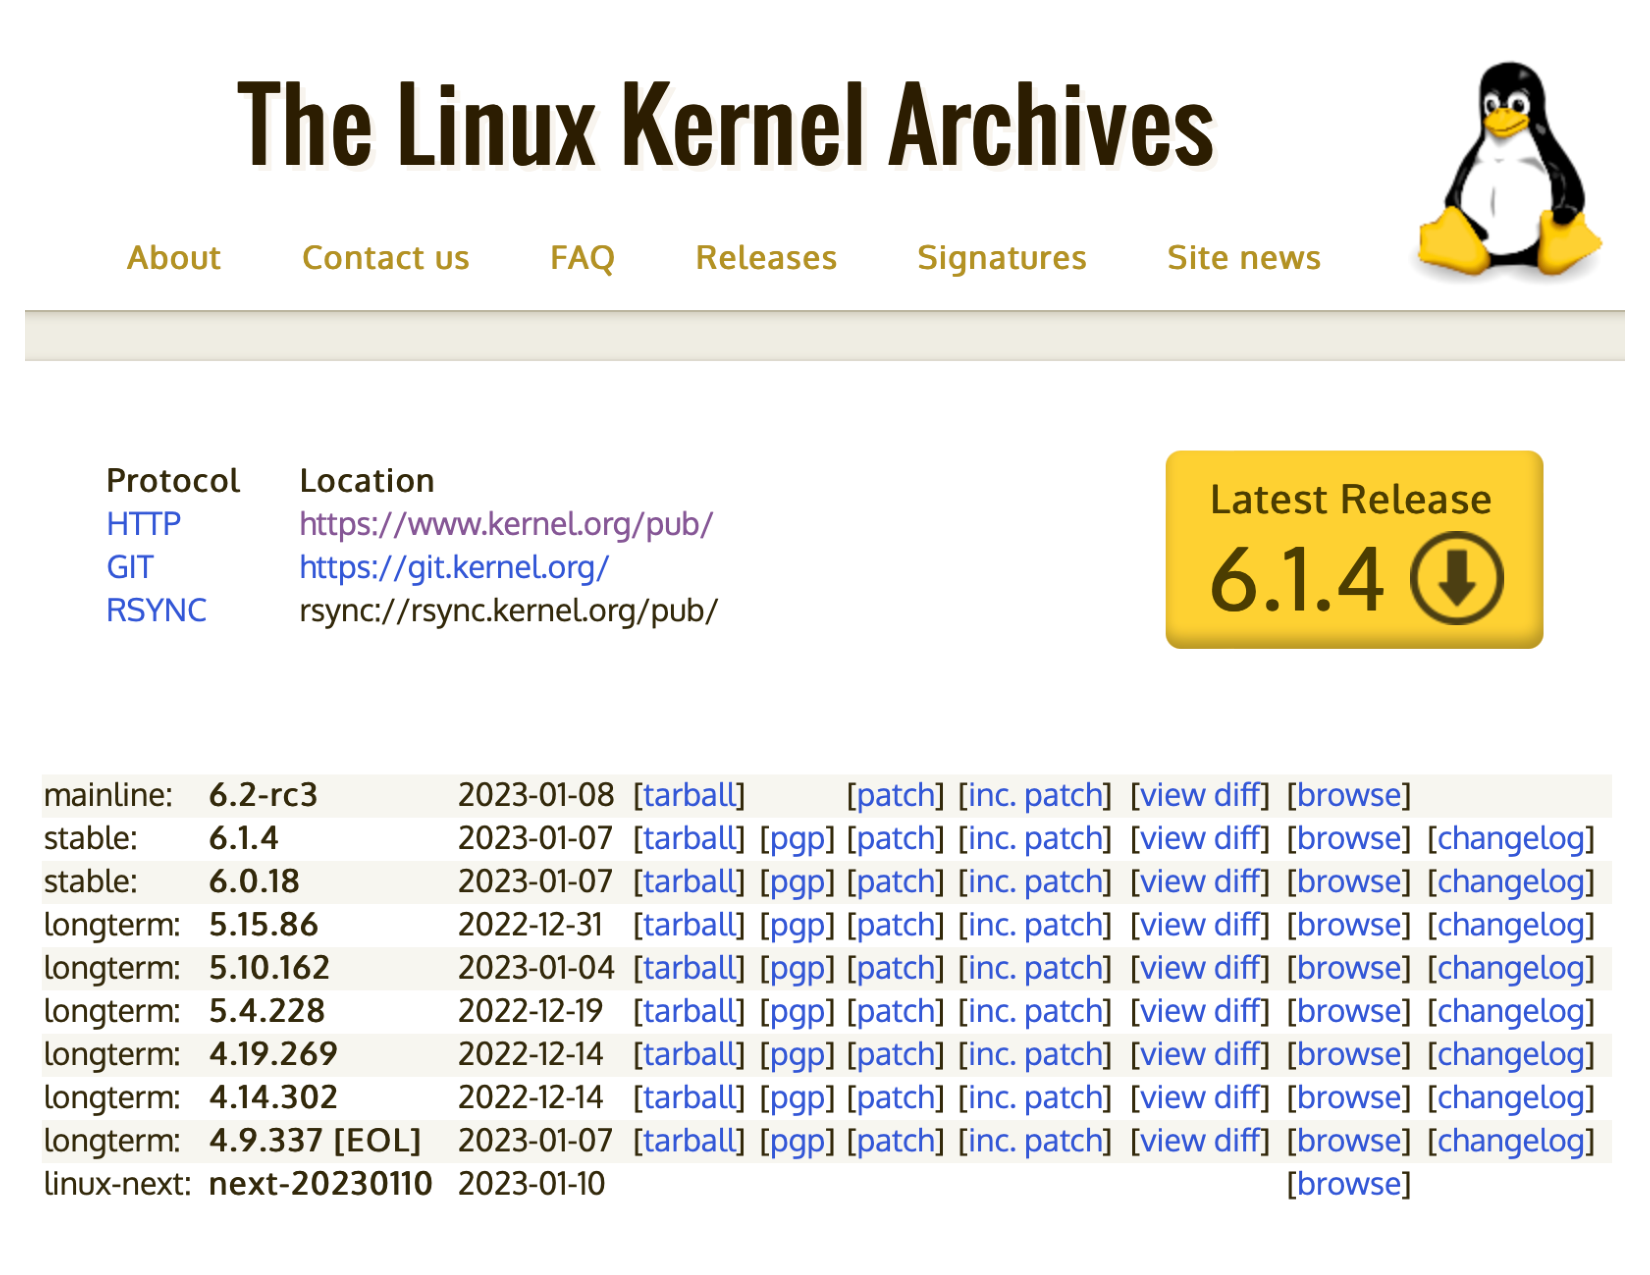
\includegraphics[scale=0.4]{figures/kernel-org.pdf}
	\centering
	\caption{www.kernel.org --- home of the Linux source code}
	\label{fig:kernel-org}
\end{figure}

On the \cf{kernel.org} home page there is a link to \cf{https://docs.kernel.org}, which contains documentation covering everything from building the kernel to submitting patches to building loadable modules. There is a wealth of information here, although some of the documentation is more detailed than others and all vary as to when they were written. Don't take everything there as gospel. The source code is always has the final say.

This chapter won't cover all of the kernel source code since only a small subset is relevant to filesystem development.  However, the goal of this section is to give you an overview of what everything is and where different subsystems can be found. Starting at the top level of the kernel source tree, these are the directories that you will see:

% describe the layout of the source code

\begin{itemize}
	\item \cf{Documentation} -- there are 8,579 files in this directory and subdirectories at the time of writing
		(the 6.3.3 kernel).
		Some of the documentation is quite old but it's still a good place to start in order to find information. You will see
		a lot of \cf{.rst} files (reStructuredText -- a simple markup language). You can build the documentation yourself 
		although I found that a lot of disk space is needed to pull all the necessary packages to build it. Alternatively, and 
		to simplify things, you can go to \cf{www.kernel.org/doc/html}, locate the kernel of choice and view the 
		same documentation there.
	\item \cf{Makefile} -- the top-level makefile which is used when building the kernel. This book doesn't describe
		much about kernel builds other than when discussing \cf{kgdb} in section \ref{kgdb}. For detailed
		information about building the kernel, submitting patches and so on, refer to \cf{https://docs.kernel.org} 
		or search for information specific to the distribution that you are using.
	\item \cf{arch} -- architecture-specific source code for the just over twenty different platforms that Linux supports /
		has supported. You will see a directory for each different architecture, for example, \cf{x86}, \cf{arm64}
		and \cf{s390}. System call entry points can be found under \cf{arch/x86/entry/syscalls}. Platform independent 
		system call handling will be described below in section \ref{syscalls}. Platform initialization code (assembler and C) 
		as well as lower-level memory management and interrupt handling code can be found within these directories.
	\item \cf{block} -- generic code for the kernel \textit{block layer}. To see source code for each of the block device 
		drivers, refer to the directories under \cf{drivers/block}.
	\item \cf{certs} -- kernel module signing allows for cryptographically signing modules during installation 
		and then checking these signatures when modules are loaded. This increases kernel security 
		by disallowing the loading of unsigned modules or modules signed with an invalid key.
	\item \cf{crypto} -- an array of cryptographic functions that can be used by the kernel and kernel modules. There are also
		crypto routines in \cf{drivers/crypto} and architecture specific crypto routines. For example, you
		can find Intel AES-NI crypto code in \cf{arch/x86/crypto}.
	\item \cf{drivers} -- contains the majority of the device driver code in driver-specific directories. As an example, you
		will see \cf{usb} and \cf{bluetooth} directories. Some directories contain source code that is generic
		for the hardware type (\cf{drivers/scsi} for example) together with drivers for specific hardware cards.
	\item \cf{fs} -- filesystem independent (VFS -- Virtual File System) and filesystem dependent code. Files 
		at the top level of this directory are filesystem dependent. Each filesystem has its own directory, for 
		example, \cf{fs/ext4} and \cf{fs/xfs}. This is the main place to look at when studying filesystems.
	\item \cf{include} -- header files and almost 6,000 of them. These are not the only header files
		in the kernel source. A quick "\cf{find . -name '*.h'}" will show header files scattered
		throughout the source tree. Most of the header files in this directory are used by generic
		kernel subsysttems or drivers and filesystems.
	\item \cf{init} -- a small amount of code that is executed during startup of the Linux kernel. Look for the
		function \cf{start\_kernel()} in \cf{init/main.c} if you wish to study some of the early code paths. This function 
		performs early initialization tasks including creating a kernel thread which ultimately becomes \cf{/sbin/init}.
	\item \cf{ipc} -- System V IPC (Inter-Process Communication), source code for handling shared memory segments, 
		semaphores and message queues. 
	\item \cf{kernel} -- 80,000+ lines of kernel code that handles everything from process management to signal 
		handling to reboot to system call handling (after entry through architecture-dependent code 
		in \cf{arch}). Most file names give a hint as to what the source code inside does.
	\item \cf{lib} -- generic routines that are of use to all kernel subsystems can be found here. There is
		everything from crypto and string operations to debugging routines and linked list management.
	\item \cf{mm} -- memory management which will be described later in the book in some detail since there is a lot 
		of interaction between the virtual file subsystem and the memory management subsystem. For memory management
		code that's architecture-specific, see \cf{arch/<platform>/mm}.
	\item \cf{net} --- everything networking related. 
	\item \cf{samples} -- various sample pieces of code. For example, inside the \cf{ebpf} directory there are tests for eBPF and
		files under \cf{kobject} contains code to create a simple subdirectory in \cf{sysfs}. 
	\item \cf{scripts} -- there are a lot of makefiles and scripts. One such example is the directory \cf{scripts/gdb/linux} 
		which contains Python helper scripts which will be described in section \ref{gdb-helper} and used in the many
		\cf{gdb} examples  throughout the book.
	\item \cf{security} -- security-related source code including support functions for SELinux and
		AppArmor. 
	\item \cf{sound} -- all things sound related including drivers and the \textit{Advanced Linux Sound 
		Architecture} (ALSA) which provides audio and MIDI functionality.
	\item \cf{tools} -- an array of different tools for use with x86 CPU power management, thermal monitoring, eBPF, tracing
		and PCI support.
	\item \cf{usr} -- source code which builds a \cf{cpio} archive containing a temporary root filesystem image 
		(referred to as the \cf{initramfs} image). This is used for an early user-space file hierarchy on to which the real
		root filesystem will be mounted early during system initialization.
	\item \cf{virt} --  source code for handling virtualization, specifically KVM (Kernel Virtual Machine). This is located 
		under \cf{virt/kvm}.
\end{itemize}

\noindent
It can be quite daunting to look at this vast amount of source code but to analyze filesystem and filesystem-related code, you only need to look at a relatively small number of files in a few directories. The following sections will help guide you as to where these files are and also describe a set of good tools to use to help with browsing the source code.

\section{User-Space vs Kernel-Space}

Before digging further into the kernel source, this is a good time to describe the difference between user-space and kernel-space. The latter is also called "\textit{running in the kernel}" or "\textit{operating in kernel-mode}".

Each Linux process runs in its own address space. The process address space is a protected range of memory addresses in which a Linux process runs supported by underlying hardware mechanisms such that one process is unable to access memory addresses of another. Figure \ref{fig:process-address-space} shows the layout of two different Linux processes in memory. The kernel is \textit{mapped} into the address spaces of all process and at the same location. All memory addresses in the kernel-space are not accessible by the program that is running in user-space. Any attempt is made to access a kernel address will result in a \textit{segmentation violation}. If this happens, the process will receive a \cf{SIGSEGV} signal and terminate. A process can only enter the kernel voluntarily by invoking one of the many system calls which the kernel will then service. 

Everything that is not in kernel-space is considered to be in user-space. This includes the program TEXT (the program's executable instructions) which is at the lower end of memory. Arguments passed to the program and the program's environment variables are at the higher portion of user-space. The stack grows down in memory as more functions are called and any data allocated via \cf{malloc(2)} is taken from the heap which grows up towards the stack. It is from the heap that most file I/O will occur since processes will generally allocate memory buffers dynamically.

Each time a call is made to fork a new process, the new process is started in its own address space. A call is then typically made to \cf{execve(2)} to execute a new binary (typically via one of the \cf{exec(3)} family of functions). For the differences between the parent process and the child process following a fork, refer to the \cf{fork(2)} manpage.

\begin{figure}[h]
	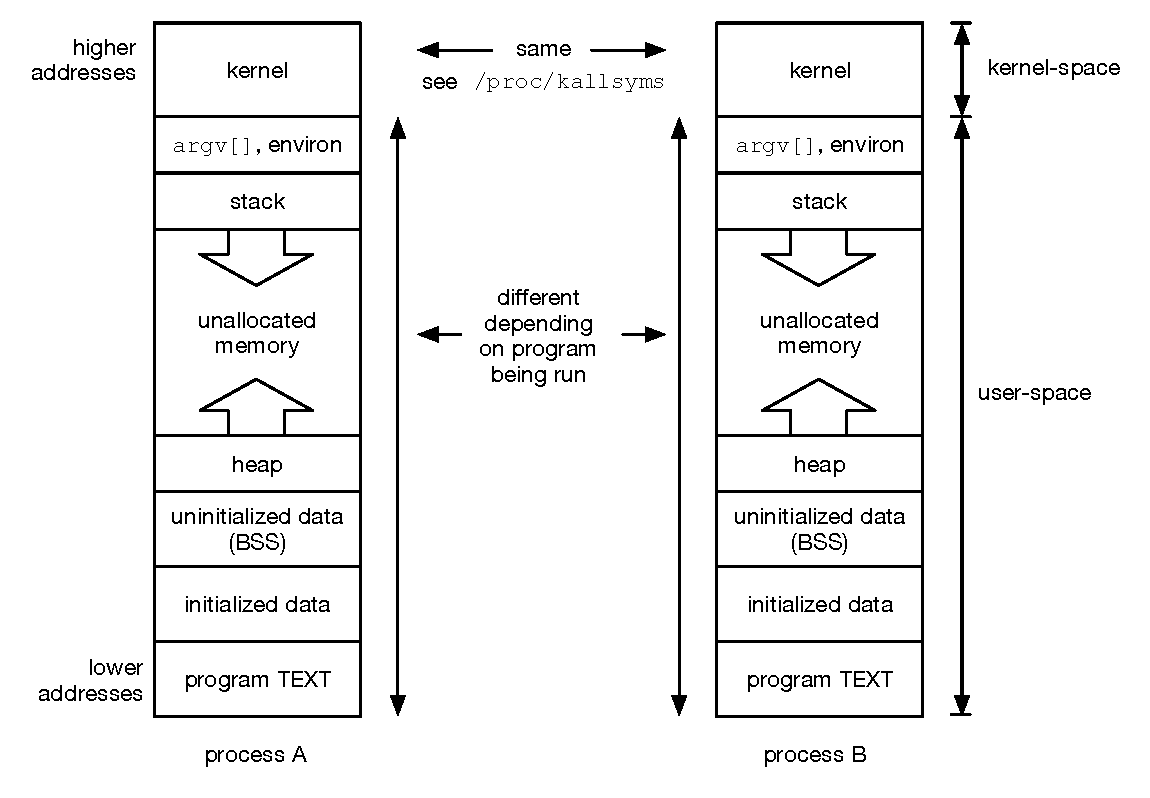
\includegraphics[scale=0.6]{figures/process-address-space.pdf}
	\centering
	\caption{Process address space showing user-space and kernel-space}
	\label{fig:process-address-space}
\end{figure}
 
It would be fun to explore the process address space here in more detail but that's a topic for another book or blog post. In short, just recognize that each process has its own, unique address space that is separate from all other processes, the kernel is mapped into all address spaces, user programs cannot access kernel addresses directly but can enter the kernel intentionally by invoking a system call.

%%%%%%%%%%%%%%%%%%%%%%%%%%%%%%%%%%%%%%%%%%%%%%%%%%%%%%%%%%%%%

\section{The System Call Interface}\label{syscalls}

This section shows how applications enter the kernel through invoking \textit{system calls}. The goal is to give readers a good place to start exploring execution paths through the kernel in response to familiar system calls that a program invokes such as \cf{open(2)}, \cf{read(2)} and \cf{stat(2)}.

A \textit{system call handler} is nothing more than a C function that operates in kernel space and calls other functions as needed. But the means of getting to this C function is somewhat complex and depends on the architecture on which the program is running. Consider figure \ref{fig:syscall-kernel} which shows the path from a everyone's favorite "\textit{Hello world!}" C program which calls \cf{printf(3)} which ends up in a call to the \cf{ksys\_write()} system call handler in the kernel. The program calls the standard library routine \cf{printf(3)} which in turn will invoke the \cf{write(2)} system call in order to write the string "\cf{hello world\textbackslash n}" to \cf{stdout}.

\begin{figure}
	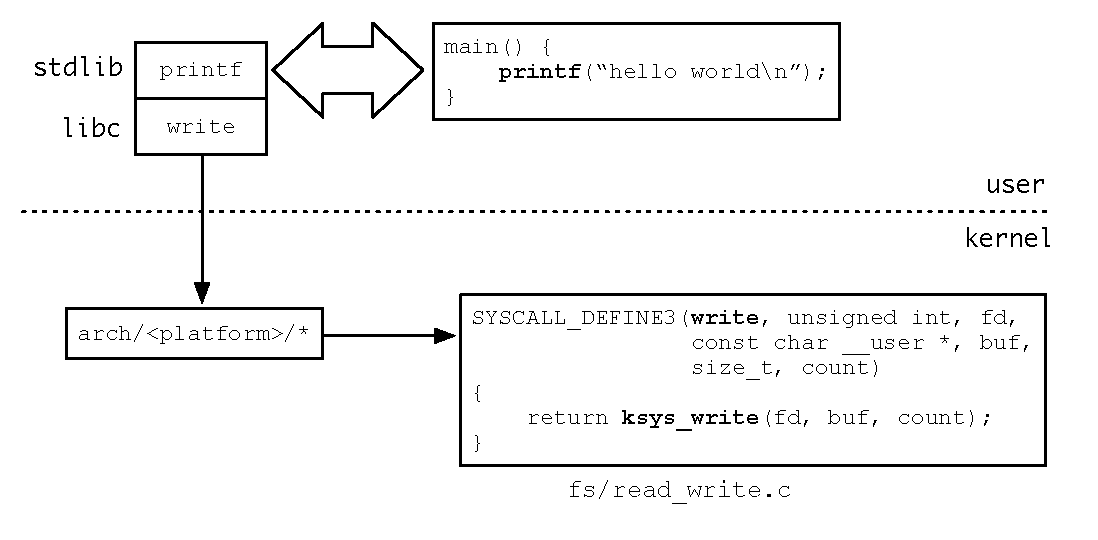
\includegraphics[scale=0.6]{figures/syscall-kernel.pdf}
	\centering
	\caption{Entering the kernel through the \cf{write(2)} system call}
	\label{fig:syscall-kernel}
\end{figure}

The details of how system calls are handled on each architecture won't be described in detail here but what follows are the steps taken on the x86\_64 architecture by the standard library (\cf{libc}) to enter the kernel for our "\cf{printf(Hello world!$\backslash$n");}" program. Arguments are passed into the kernel via CPU registers. If there are more than six arguments, the remaining arguments as pushed onto the stack.

\begin{quote}
- Store "1" in \cf{\%rax} ("1" is the system call number for the "write" system call)

- Store argument 1 in \cf{\%rdi} (in this case it will be "1" for \cf{stdout})

- Store argument 2 in \cf{\%rsi} (a pointer to the string "\cf{hello world\textbackslash n}")

- Store argument 3 in \cf{\%rdx} (the length of the string "\cf{hello world\textbackslash n}")

- Call the x86\_64 instruction "\cf{syscall}" to enter the kernel
\end{quote}

\noindent
For the Intel architecture, in the directory \cf{arch/x86/entry/syscalls}, there are two files which contain system call tables for both the 32-bit and 64-bit architectures. These files are \cf{syscall\_32.tbl} and \cf{syscall\_64.tbl} respectively. Here are the first few lines of \cf{syscall\_32.tbl}:

\begin{lstlisting}
0   i386    restart_syscall sys_restart_syscall
1   i386    exit            sys_exit
2   i386    fork            sys_fork
3   i386    read            sys_read
4   i386    write           sys_write
\end{lstlisting}

\noindent
You can see \cf{sys\_write} has the value of "4" which is different to the x86\_64 example above. On contrast, here are the first few lines of \cf{syscall\_64.tbl} for which the \cf{write(2)} system call is at position "1":

\begin{lstlisting}
0   common  read            sys_read
1   common  write           sys_write
2   common  open            sys_open
3   common  close           sys_close
4   common  stat            sys_newstat
\end{lstlisting}

\noindent
For further details on how system calls on x86 are handled I'd recommend reading the \textit{0xax} article "\textit{System calls in the Linux kernel. Part 1.}":

\begin{table}[h]
\begin{tabular}{lcl}
\parbox[r]{0.5in}{
\includegraphics[scale=0.15]{figures/url.png}} & \parbox[l]{0.55in}{URL \arabic{urls}} & \parbox[l]{3in}{\cf{https://tinyurl.com/rb3z8kds}}
\end{tabular}
\end{table}
\stepcounter{urls}
% https://0xax.gitbooks.io/linux-insides/content/SysCall/linux-syscall-1.html

\noindent
which explains how system calls are handled on the x86 platform in great detail. It shows an assembler version of "\textit{Hello world}", describing the path through to the architecture-specific areas of the kernel and into the C system call handling functions. 

\subsection{System Calls for File / Filesystem Activity}

There are a lot of system calls, in fact 322 for x86\_64 and 358 for x86. How many of these are related to filesystem activity? File / filesystem related system calls can be found in the \cf{fs} directory at the top level of the Linux kernel source tree. To get a rough idea of the number of file / filesystem related system calls, head into the \cf{fs} directory and run the following:

\begin{lstlisting}
$ [*\bfseries grep SYSCALL\_DEFINE3 *c | wc -l *]
56
\end{lstlisting}

\noindent
The actual number is a little less but this should help you get an idea of how many file / filesystem operations the kernel supports for applications.

Generally speaking, the easiest way to find the specific functions is to run "\cf{grep}" and you'll see that the file/filesystem functions are spread across 16 files. Here are some examples where \cf{grep} is run to look for specific function calls.

\begin{lstlisting}
$ [*\bfseries grep 'SYSCALL\_DEFINE3(write' *.c*]
read_write.c:SYSCALL_DEFINE3(write, unsigned int, fd, ...
read_write.c:SYSCALL_DEFINE3(writev, unsigned long, fd, ...
$ [*\bfseries grep 'SYSCALL\_DEFINE3(read' *.c *]
read_write.c:SYSCALL_DEFINE3(read, unsigned int, fd, ...
read_write.c:SYSCALL_DEFINE3(readv, unsigned long, fd, ...
stat.c:SYSCALL_DEFINE3(readlink, const char __user *, path, ...
$ [*\bfseries grep 'SYSCALL\_DEFINE3(fcntl' *.c*]
fcntl.c:SYSCALL_DEFINE3(fcntl, unsigned int, fd,  ...
fcntl.c:SYSCALL_DEFINE3(fcntl64, unsigned int, fd, ...
fcntl.c:COMPAT_SYSCALL_DEFINE3(fcntl64,  ...
fcntl.c:COMPAT_SYSCALL_DEFINE3(fcntl, unsigned int, fd, ...
\end{lstlisting}

\noindent
Most of these top-level functions don't do a great deal other than call other kernel functions. For example, in the case of the \cf{write(2)} system call, a call is made to \cf{ksys\_write()} as follows:

\begin{lstlisting}
SYSCALL_DEFINE3(write, unsigned int, fd, const char __user *, 
                buf, size_t, count)
{
    return ksys_write(fd, buf, count);
}
\end{lstlisting}

\noindent
There are 76 source code files in the \cf{fs} directory and over 90,000 LOC but the names of the files generally give a good hint as to what functionality they provide. For example:

\begin{itemize}
	\item \cf{open.c} -- contains source code for the \cf{open(2)} system call and other operations generally associated 
		with opening a file such as  \cf{ftruncate(2)} and the different file ownership change system calls 
		(\cf{chown(2)}, \cf{lchown(2)} etc), 
	\item \cf{read\_write.c} -- the code for \cf{read(2)}, \cf{write(2)} and vectored read / write system calls.
	\item \cf{readdir.c} -- system calls for reading directories including \cf{getdents64(2)}.
\end{itemize}

\noindent
There are several ways to browse through the kernel source but the best way will depend on your own personal preferences. Some people are happy with "\cf{cd}" and "\cf{grep}" but there are several tools that can help or at least give different options. Three such tools will be described in the following sections.

\subsection{Using \cf{vim} and \cf{ctags} to Browse the Kernel Source}

I remember the first time a colleague looked at me in surprise and said "\textit{You don't use tag stacking?}". I learned very quickly and have been using it for 30 years now. Most editors can make use of \cf{ctags(1)} but the program was originally built several decades ago to be used with \cf{vi(1)}.  What are ctags? From the manpage:

\begin{quote}
\textit{The ctags and etags programs (hereinafter collectively referred to as
       ctags, except where distinguished) generate an index (or "tag") file for
       a variety of language objects found in file(s).  This tag file allows
       these items to be quickly and easily located by a text editor or other
       utility. A "tag" signifies a language object for which an index entry is
       available (or, alternatively, the index entry created for that object).}
\end{quote}

\noindent
The following example generates a tags file for the whole of the Linux kernel source code. To do this, simply head to the top level directory of the source code and run the "\cf{ctags}" command:

\begin{lstlisting}
$ [*\bfseries cd linux-6.3.3*]
$ [*\bfseries ctags -R **]
\end{lstlisting}

\noindent
This will create a very large file (for the 6.3.3 sources it's 1,067,091,840 bytes - ouch!).

Once you have the tags file, navigate to the top level Linux source tree and enter your favorite editor using the option to specify a tag. In \cf{vi} pass the \cf{-t} option together with the function or global variable that you're looking for. The following command will open \cf{vi} in \cf{fs/read\_write.c} with \cf{ksys\_write()} in the center of the screen.

\begin{lstlisting}
$ [*\bfseries vi -t ksys\_write*]
\end{lstlisting}

\noindent
Note that you need to be in the directory where the tags file is located. You can also search for global variables too so:

\begin{lstlisting}
$ [*\bfseries vi -t file\_systems*]
\end{lstlisting}

\noindent
will open \cf{vi} in \cf{fs/filesystems.c} at the place where the \cf{file\_systems} global variable is defined.

I typically have this one-liner in my \cf{.bashrc} file:

\begin{lstlisting}
alias linux='cd ~/src/linux-6.3.3 ; pwd'
\end{lstlisting}

\noindent
to get me to the top of the current source tree that I'm using. I can then run "\cf{vi -t}" to enter the file at the place I want.

Another option is to build a little script that displays various routines. The following script switches to the top of the kernel source tree where it assumes you have a tags file and then enters \cf{vi} using a tag that you choose. The advantage here is that once inside the file, you can now use tag stacking to move through the kernel source from one function to another. 

Here is a shorter version of the \cf{bash} script. It's very simple and obviously you can put any function or global variable in here.

\begin{lstlisting}
TAGS_DIR=~/src/linux-6.3.3

echo "
1 - open
2 - read
3 - write
4 - readlink

a - task_struct
b - super_operations

q - quit
"

cd $TAGS_DIR
while :
do
    /bin/echo -n "System call? "
    read choice
    case $choice in
        1) vi -t do_sys_open ;;
        2) vi -t ksys_read ;;
        3) vi -t ksys_write ;;
        4) vi -t do_readlinkat ;;
        a) vi -t task_struct ;;
        b) vi -t super_operations ;;
        q) break ;;
        *) echo "Invalid choice"
    esac
done
\end{lstlisting}

\noindent
Now that you can get in to a file at the location of the system call handler you've been looking for, it's time to cover how tag stacking works so you can search through the code from one function to the next. Regardless of where you are in the file, if you want to go to the location of the tag where the cursor points to and then back again to the current file and location, use the following two commands in order:

\begin{itemize}
	\item \cf{Ctrl + ]} -- Move to the file where the tag under cursor is located (function, global variable etc). This is 
		identical to running "\cf{vi -t}"  specifying the tag name from the command line.
	\item \cf{Ctrl + t} -- Move back to the previous file/position.
\end{itemize}

\noindent
For example, in figure \ref{fig:tag-stacking} we entered this file with "\cf{vi -t ksys\_write}" and the cursor is on
the function name \cf{vfs\_read()}. By hitting "\cf{Ctrl + ]}", \cf{vi} will take you to the location of \cf{vfs\_read()}. It happens to be in the same file but if it was a different file, you'd enter that file instead. If you then hit "\cf{Ctrl + t}" you will go back to the file/location where you started.

\begin{figure}
	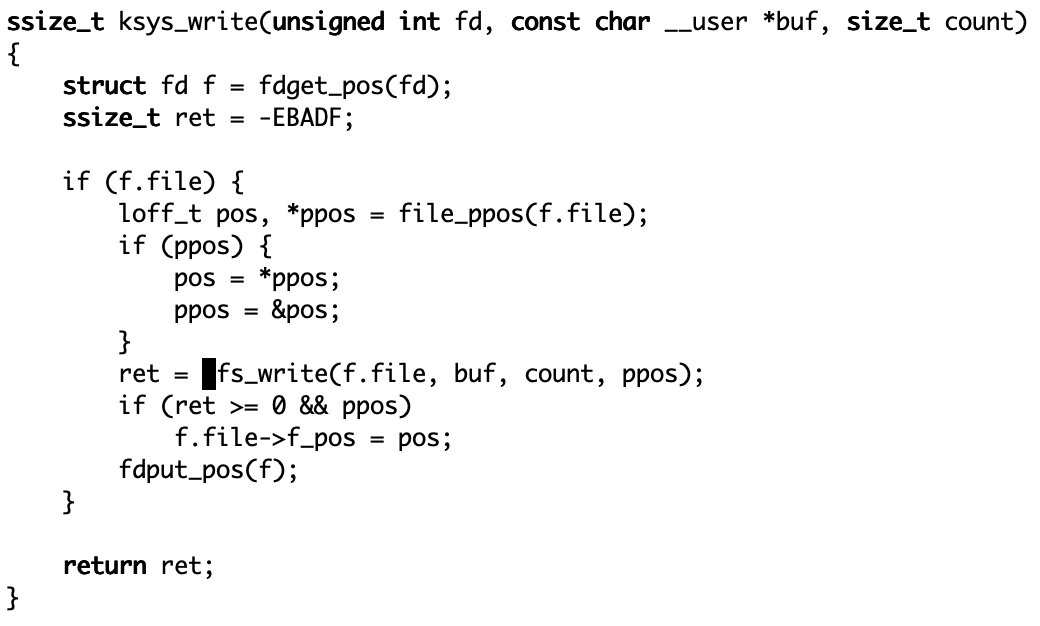
\includegraphics[scale=0.6]{figures/tag-stacking.png}
	\centering
	\caption{Using tag-stacking to navigate through the kernel source code}
	\label{fig:tag-stacking}
\end{figure}

The current tag stack is the list of all places in the source tree you have moved to through repeated calls to "\cf{Ctrl + ]}". You can view the current tag stack by typing "\cf{:tags}" in \cf{vi}. See figure \ref{fig:tag-stacking-2} for an example. This shows going from \cf{vi -t ksys\_write} to \cf{vfs\_read()} and then to \cf{rw\_verify\_area()}.

\begin{figure}[h]
	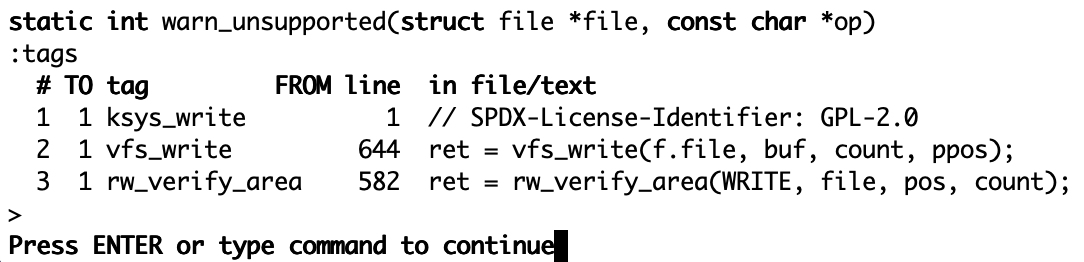
\includegraphics[scale=0.6]{figures/tag-stacking-2.png}
	\centering
	\caption{Current tag stack}
	\label{fig:tag-stacking-2}
\end{figure}

I've tried some of the newer editors and have struggled to move around files as quickly as I can with \cf{vi} and tag stacking.

\subsection{Using \cf{cscope} to Browse the Kernel Source}

Another excellent tool to use, especially in conjunction with \cf{vi} and tag stacking, is the \cf{cscope(1)} command which has been around since the early 1980s. It's a tool I've used for over thirty years and have used extensively while writing this book. Notes about the early history of \cf{cscope} can be found here:

\begin{table}[h]
\begin{tabular}{lcl}
\parbox[r]{0.5in}{
\includegraphics[scale=0.15]{figures/url.png}} & \parbox[l]{0.55in}{URL \arabic{urls} -- } & \parbox[l]{3in}{\cf{https://tinyurl.com/ywce8h9n}}
\end{tabular}
\end{table}
\stepcounter{urls}
% https://cscope.sourceforge.net/history.html

I particularly enjoyed reading the goals behind starting the project:

\begin{quote}
\textit{Joe Steffen first started writing cscope in the early 1980's as an aid for his own work. It started as little more than a set of shell scripts containing greps and seds. It became clear to Joe that this was not going to work on large projects (say, more than 20 or so files, which was a large project on a PDP-11!) as most of the time consumed was in parsing the C source code over and over again. So he wrote a C program that did the grunt work of parsing into a tagged database, and then presented the screen with common searches. The tagged database was updatable and saved between sessions. Productivity soared!}
\end{quote}

\noindent
Imagine that -- a project with 20 or so files? Today, the Linux kernel source tree now has close to 26 million files. Of course \cf{grep} is still very useful so some things don't change.

History lesson beside, the first time you run \cf{cscope} you will need to generate the cross-reference database as shown below. The command must be run from the top kernel source directory:

\begin{lstlisting}
$ [*\bfseries cd linux-6.3.3*]
$ [*\bfseries cscope -Rk **]
\end{lstlisting}

\noindent
Since the kernel source is quite large, this takes quite a while and the database comes in at over just over 1 GB. Thus you'll need over 2 GB of free space for using "\cf{cscope}" and "\cf{ctags}". The "\cf{R}" option instructs \cf{crash} to recurse through all directories and the "\cf{k}" option (Kernel Mode) will turn off using the default include directory (\cf{/usr/include}) when building the database, since when building the kernel, these include files won't be used. Only header files within the kernel source tree are used since header files in \cf{/usr/include} will likely be for a different kernel release. In the Linux source tree, the \cf{include} directory used during kernel builds is at the top level of the source tree. 

Once the database has been generated or on subsequent runs, you will see output similar to what is shown in figure \ref{fig:cscope-1}. The \cf{cscope} version will be displayed at the top of the screen together with a note to let you know that you can press "\cf{?}" at any time to get help:
 
 \begin{figure}[h]
	\centering
	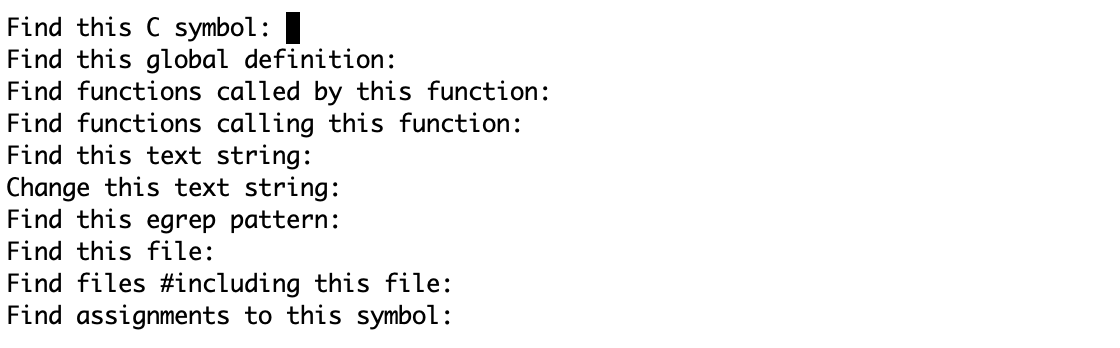
\includegraphics[scale=0.6]{figures/cscope-1.png}
	\caption{The main \cf{cscope} screen}
	\label{fig:cscope-1}
\end{figure}

Everything is set up such that the cursor is on the line where you can search for a symbol so all you have to do is enter the symbol you are looking for and press the return key. For example, after typing "\cf{ksys\_read}" and pressing "RETURN", the results will be displayed at the top of the screen as shown in figure \ref{fig:cscope-2}.

\begin{figure}
	\centering
	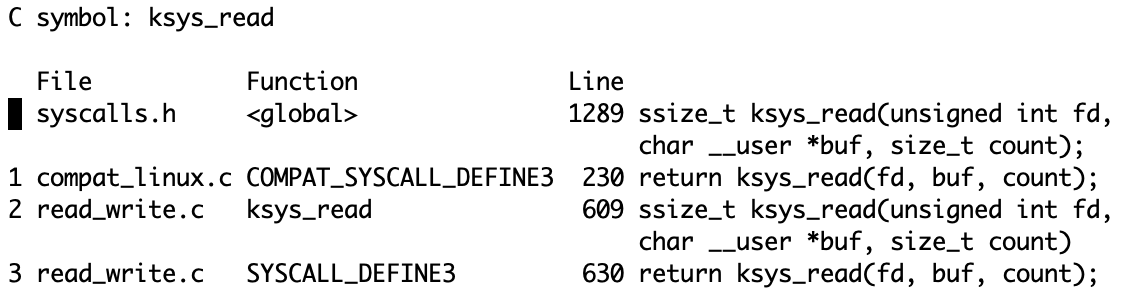
\includegraphics[scale=0.6]{figures/cscope-2.png}
	\caption{The \cf{cscope} results of searching for \cf{ksys\_read}}
	\label{fig:cscope-2}
\end{figure}

For each search item displayed you can press the number key shown on the left-hand-side to enter the file at that location. In this example, press '\cf{2}' to enter \cf{read\_write.c} at the location where the function \cf{ksys\_read()} is located. Or you can use the arrow keys to move between items displayed and just press "RETURN". If there are more items than can be displayed on a single screen, use the space bar to go to subsequent screens. The "TAB" key toggles between the search results and the menu at the bottom of the screen. "\cf{Ctrl + d}" exits \cf{cscope}. 

While in menu mode, if you use the arrow keys to move down to "\cf{Find this global definition}", type \cf{ksys\_read} and press the return key, \cf{cscope} will locate the symbol and enter the file at the correct location. If you are looking for a function that is called by many other functions, the list of hits at the top of the screen could be several pages long. Searching for the global definition can save time searching.

Next time you run \cf{cscope} just add the \cf{-d} option to instruct it not to regenerate the database again. Unless of course some of the source code files have changed. If the database needs to be generated again, it should be faster than the first time it's generated.

Now the best part of using \cf{cscope} is to combine it with your favorite editor and use tag stacking. Then you have the best of all worlds since you can search easily, locate the function of your choice and move down through functions it calls.

%------------------------------------------------------------------------------------------------------------------------------------------------------------------

\subsection{Using Elixir to Browse the Kernel Source}

Elixir is a cross reference tool for the Linux source code hosted by embedded Linux provider Bootlin. It doesn't just support a specific version of the kernel but every version that exists all the way back to day one and up to the most recent development kernels. Everyone has their own way of navigating through source code using their favorite editor and using tools such as \cf{ctags} but sometimes it's nice just scroll through a page of source code using the mouse. You can find Elixir by pointing the browser to \cf{elixir.bootlin.com} to get to the latest sources or using the following link. Alternatively just search for "elixir linux" in your favorite browser.

\begin{table}[h]
\begin{tabular}{lcl}
\parbox[r]{0.5in}{ 
\includegraphics[scale=0.15]{figures/url.png}} & \parbox[l]{0.1in}{\arabic{urls}} & \parbox[l]{3in}{\cf{https://tinyurl.com/447v7urs}}
\end{tabular}
\end{table}
\stepcounter{urls}
% https://elixir.bootlin.com/linux/latest/source

\noindent
Figure \ref{fig:elixr-1} shows an example of using Elixir and displaying the results of searching for the symbol \cf{ksys\_write}. In this example, we are searching through the 6.1.4 source code tree. You can change which Linux kernel version to search by selecting the version on the left hand side of the screen.

\begin{figure}
	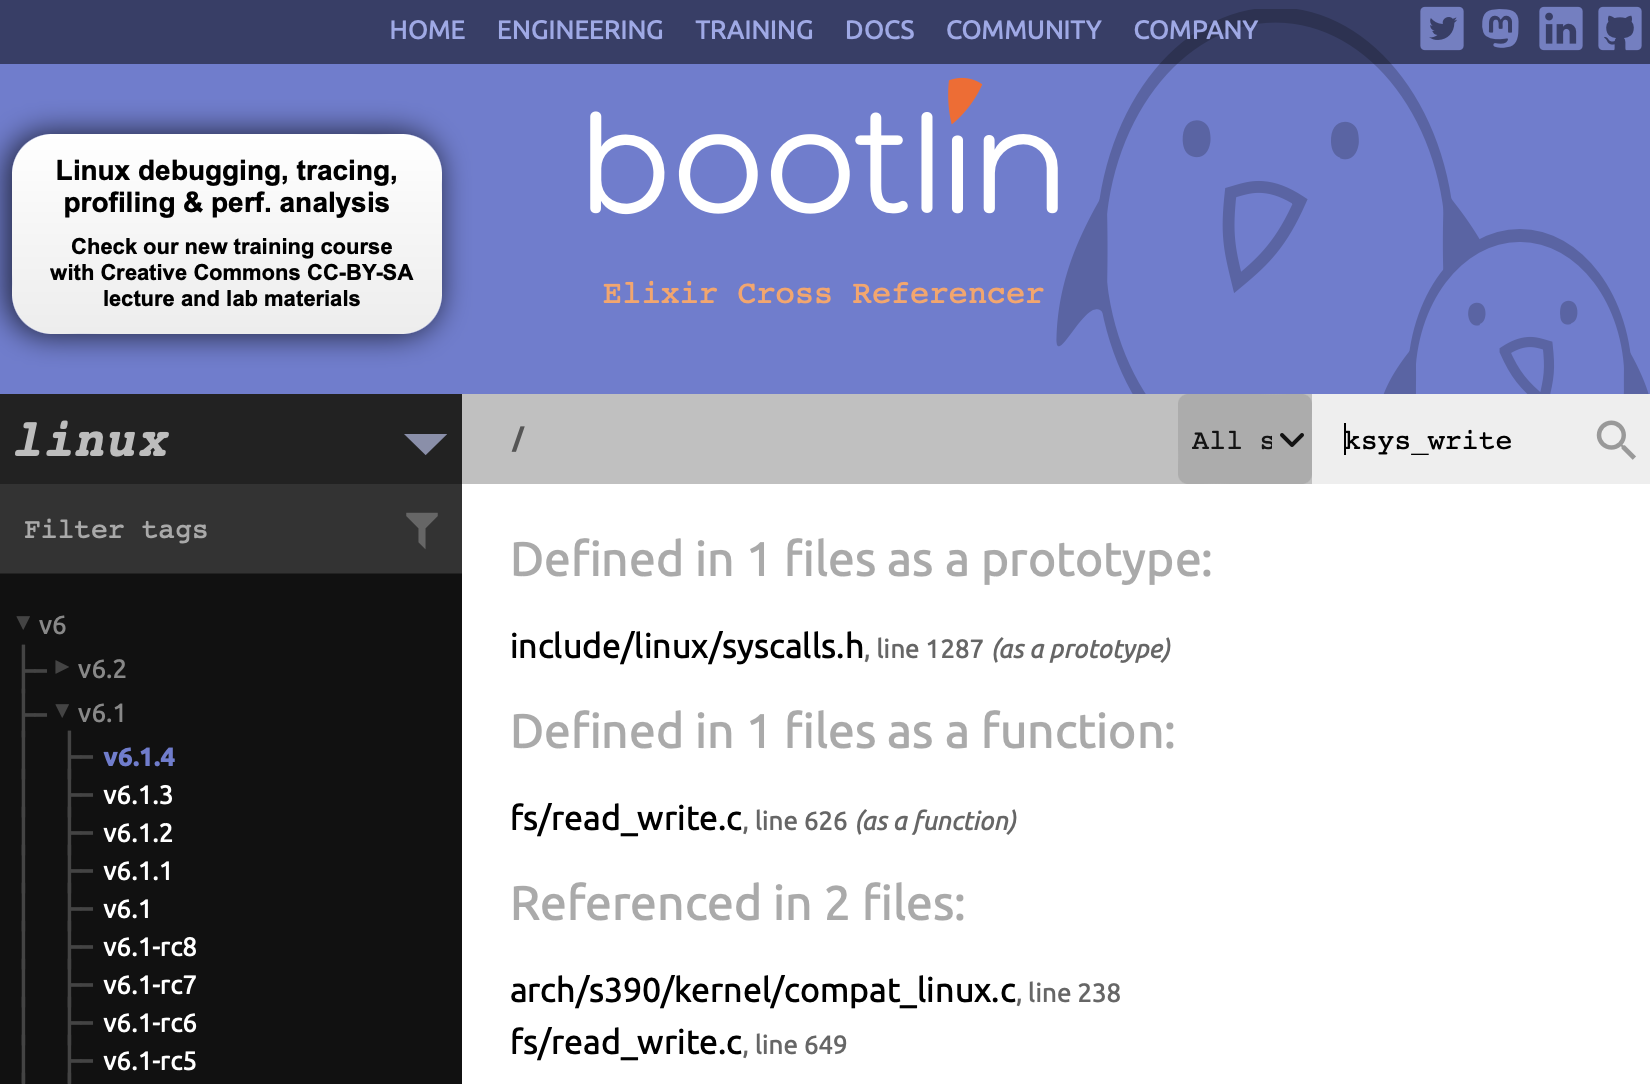
\includegraphics[scale=0.4]{figures/elixr-1.png}
	\centering
	\caption{Elixir search for the function \cf{ksys\_write}}
	\label{fig:elixr-1}
\end{figure}

Figure \ref{fig:elixr-2} shows the source code for our symbol. As well as typing the name of something to search for in the \textit{All symbols} search bar you can also click on function names and global variables when the source code is being displayed.

\begin{figure}
	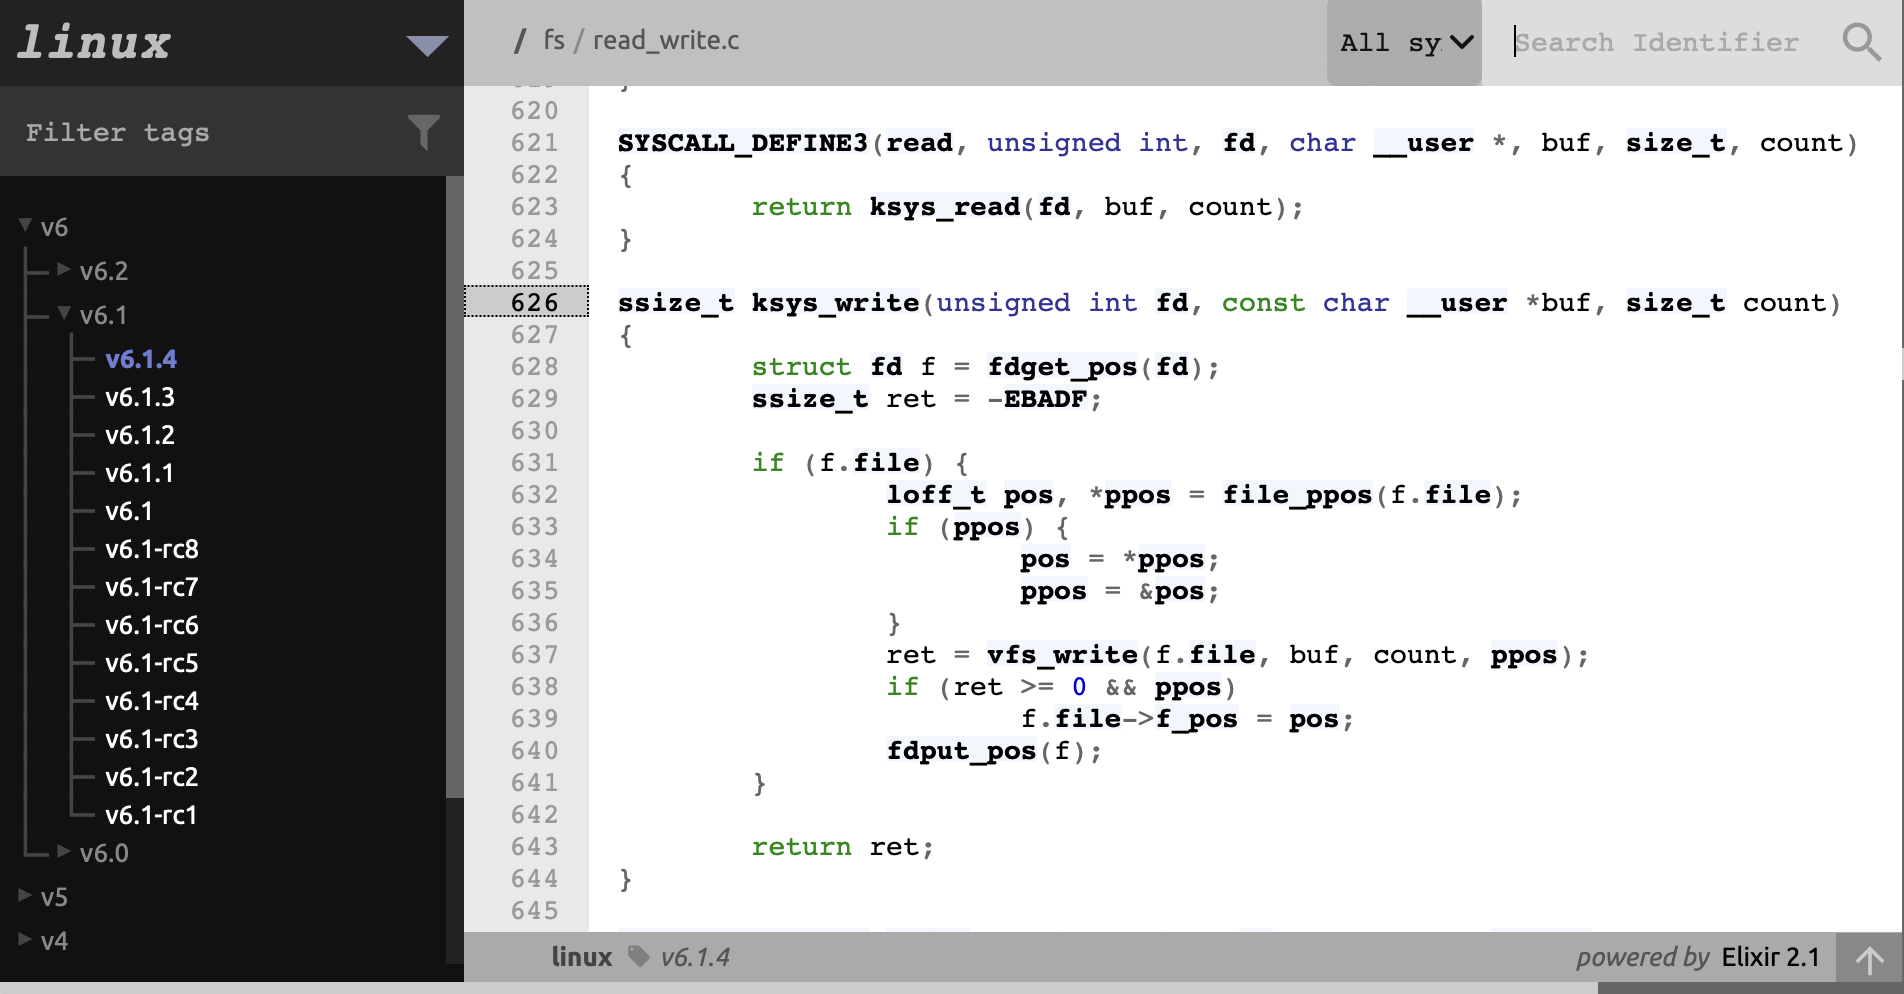
\includegraphics[scale=0.4]{figures/elixr-2.png}
	\centering
	\caption{Elixir displaying the source code for the selected function}
	\label{fig:elixr-2}
\end{figure}

You can also use Elixir on other source code projects including \cf{glibc}. Just click the arrow on the right hand side of "Linux" towards the top left of the page and a number of other projects will be displayed.


%------------------------------------------------------------------------------------------------------------------------------------------------------------------

\subsection{Maintaining Your Own Notes}

Of course you don't need to rely on all of the tools shown here for browsing the kernel source. You will develop your own methods of browsing the kernel source over time based on your preferences. How you keep notes is also a matter of personal choice. I have a directory of simple text files that I use \cf{vi} to add notes. You may wish to maintain one using rich-text or some other format.

I also have a file called "structures" which contains a copy of all of the Linux kernel structures that I typically look at. Even while browsing with \cf{vi} or Elixir, I'm usually following a code path and like to have the file close by for easy searching. It looks like this:

\begin{lstlisting}
------------------------------------------------------------

mount - fs/mount.h

    struct mount {
        struct hlist_node        mnt_hash;
        struct mount            *mnt_parent;
        struct dentry           *mnt_mountpoint;
        struct vfsmount          mnt;
        ....
    
------------------------------------------------------------

vfsmount - include/linux/mount.h

    struct vfsmount {
        struct dentry         *mnt_root;    
        struct super_block    *mnt_sb;   
        ....
\end{lstlisting}

\noindent
I've even formatted the structures to make it visibly easy to read since most of the Linux header files are full of compiler directives and \cf{\#ifdef}s which make the code harder to read. Searching for structures is also easy. I use "\cf{/\^{}vfsmount}" to search for "vfsmount" on the first line and that takes me right to the structure I'm looking for. You can do the same in your editor of choice.

I also use Omnigraffle on my Macbook Pro and have drawn a lot of code walkthrough figures, some of which can be found throughout the book. Perhaps pencil and paper or a tablet may be your choice of tool.

%%%%%%%%%%%%%%%%%%%%%%%%%%%%%%%%%%%%%%%%%%%%%%%%%%%%%%%%%%%%

\section{File Access Structures}

Now that you know where the filesystem code is located in the Linux kernel source tree and have some tools to navigate through the relevant filesystem system calls, we'll switch our focus to the main structures that are used for file / filesystem access. These structures are defined in the \cf{include} directory at the top of the Linux kernel source tree. The following sections will reference the relevant fields of each structure as each structure is explained but not all of the fields of each structure will be described. For some structures, there are many fields and describing them all here will just be overload and will inhibit  understanding how they are used. Other fields will be introduced as needed throughout subsequent chapters. 

To get started, consider figure \ref{fig:per-file-kernel-structures} which shows how the main structures in the kernel used for accessing files are linked together. It all starts with the \cf{task\_struct} structure, for which there is one such structure per process. 

In this figure there are some structures that are per-process only and some that are shared between all processes as indicated by the dotted line. For example, for every open file, each process needs its own file offset for reading and writing together with specific flags that it has set during an open call. This is where the \cf{file} struct comes into play. However, there may be multiple processes accessing the same file simultaneously so, although each process has distinct \cf{file} structures, they all share a common \cf{inode} structure for the file in question.

\begin{figure}[h]
	\centering
	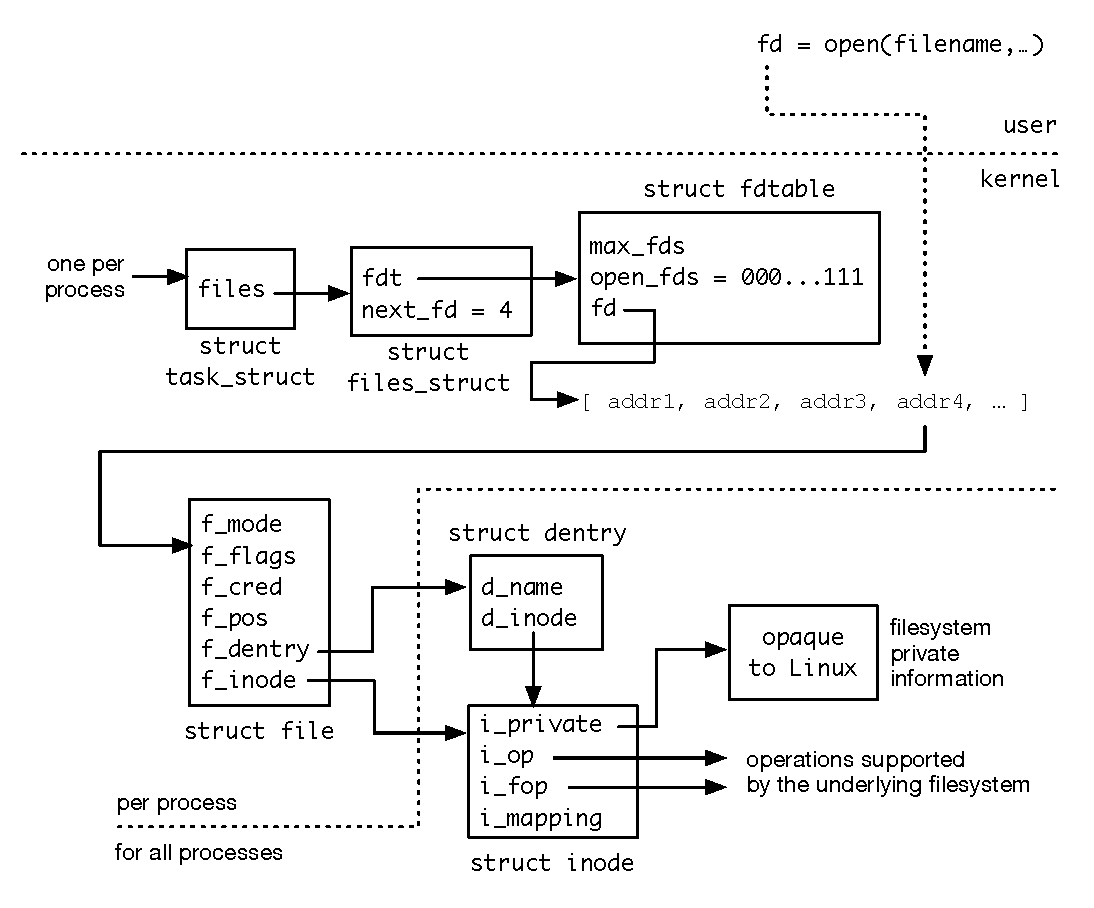
\includegraphics[scale=0.6]{figures/per-file-kernel-structures.pdf}
	\caption{Kernel structures for accessing open files}
	\label{fig:per-file-kernel-structures}
\end{figure}

%----------------------------------------------------------------------------------------------------------------------------------------------------------------

\subsection{File Descriptors}

File access starts with a file descriptor that a process gets back from \cf{open(2)} and friends. In older versions of UNIX, the file descriptor was an index into an array of pointers to "\cf{struct file}" elements held within the \cf{u\_area} structure which in turn referenced a \cf{proc} structure, similar to the Linux \cf{task\_struct}. This allowed for a fixed number of open files, a restriction that continued through to SVR3 UNIX into the early 1990s. At SCO, although we had an SVR3-based version of UNIX at the time, the limit was removed to allow for a more dynamic (and tunable) number of open files. 

This hard limit was similar in the first version of Linux which had the following field in the \cf{task\_struct} structure:

\begin{lstlisting}
struct file * filp[NR_OPEN];
\end{lstlisting}

\noindent
with \cf{NR\_OPEN} defined as 20. This meant that there was a hard coded limit of 20 open files. For most processes that's still reasonable since in a standard Ubuntu running instance, there are a relatively small number of processes with over 20 open files. 

Using a file descriptor as an index into an array pointing to \cf{file} structures was the reason that \cf{stdin}, \cf{stdout} and \cf{stderr} originally had the values of 0, 1 and 2 respectively. These numbers were used to access the first 3 elements of the file descriptor array. Regardless of how an operating system may implement POSIX file access, this convention remains intact today.

Handling file descriptors in Linux is similar today although the implementation has become more complex when handling large numbers of open files, the details of which will be described later in section \ref{fdalloc}. To get started, there are three fields in the \cf{task\_struct} which have relevance to files, filesystems and namespaces:

\begin{lstlisting}
struct task_struct {
    struct fs_struct    *fs;      /* Filesystem information: */
    ...
    struct files_struct *files;   /* Open file information: */
    ...
    struct nsproxy      *nsproxy; /* Namespaces: */
}
\end{lstlisting}

\noindent
Filesystems and namespaces will be described later but for file access, the \cf{files} field is a pointer to a \cf{files\_struct} structure for which the most relevant fields are:

\begin{lstlisting}
struct files_struct {
    struct fdtable __rcu *fdt;
    unsigned int          next_fd;
    ...
}
\end{lstlisting}

\noindent
The \cf{next\_fd} field contains the number of the next file descriptor that will be allocated. For a new process this will be 3 which is 1 above \cf{stderr}. The \cf{fdt} field points to an \cf{fdtable} structure.

%----------------------------------------------------------------------------------------------------------------------------------------------------------------

\subsection{The \cf{fdtable} Structure}

\begin{lstlisting}
struct fdtable {
    unsigned int        max_fds;
    struct file __rcu **fd;             /* current fd array */
    unsigned long      *close_on_exec;
    unsigned long      *open_fds;
    unsigned long      *full_fds_bits;
};  
\end{lstlisting}

\noindent
\textbf{Given a file descriptor, this is an efficient way to get to the \cf{file} structure in most instances. Just index into the \cf{fd} array. --- need to look to see how it works. If the fd is small and there is only one table, it's easy. If it's a larger number, can it uses the current fd array or not? Need to look}. Therefore Linux has made it efficient to handle a small number of open files while still being extensible to support a much larger number.

The \cf{max\_fds} field is set to 256 but this is just the number of file descriptors that a process can have initially and, as discussed, for most processes, this will suffice. We'll cover how greater numbers of file descriptors are managed later in section \ref{fdalloc}. It's become somewhat messy in Linux today but involves allocation of multiple \cf{fdtable} structures. \textbf{XXX -- reword all this once that work is complete}

There is one file descriptor per open instance which results from a call to \cf{open(2)}, \cf{creat(2)} for example. The \cf{file} structure however can be shared by multiple open instances (more than one file descriptor). This is achieved by calling \cf{dup(2)} which will return a new file descriptor. In this case there will be two entries in the file descriptor array (one per file descriptor) but both will point to the same \cf{file} structure.

%----------------------------------------------------------------------------------------------------------------------------------------------------------------

\subsection{The \cf{file} Structure}

The \cf{file} structure has some fields that correspond to the arguments to \cf{open(2)} call such as \cf{f\_flags} and \cf{f\_mode} as well as subsequent operations such as \cf{read(2)}, \cf{write(2)} and \cf{lseek(2)}: \textbf{XXX -- check on flags and mode when going through open code}

\begin{lstlisting}
struct file {
    struct path        f_path;   
    struct inode       f_inode;  
    atomic_long_t      f_count;  
    unsigned int       f_flags;  
    fmode_t            f_mode;   
    loff_t             f_pos;    
    struct fown_struct f_owner;  
    const struct cred  f_cred;   
    ....
}
\end{lstlisting}

\noindent
Exploring these fields:

\begin{itemize}
	\item \cf{f\_path} -- contains a pointer to the dcache dentry for this file as well as the filesystem to which this file belongs. 
		The dcache allows for fast lookups to get to a file when system calls such as \cf{open(2)} pass a pathname to search. 
		To access the file's name, the field \cf{f\_path.dentry->d\_name.name} can be used. The dcache will be described 
		below in section \ref{kstruct-dcache}.
	\item \cf{f\_inode} -- the corresponding Linux inode for the file. There may be multiple references
		to a file within a single process or from multiple processes but there will only be one Linux inode. Inodes are
		described in section \ref{inodes}.
	\item \cf{f\_count} -- a reference count for the number of file descriptors that reference  this \cf{file} structure. 
		If we open a file for the first time, \cf{f\_count} will be 1. If we then call \cf{dup(2)}, we have two file descriptors 
		referencing this same \cf{file} structure so the reference count will be 2. We'll demonstrate reference counts later on.
	\item \cf{f\_flags} -- the open flags which were passed to \cf{open(2)} and other system calls. 
	\item \cf{f\_mode} -- {\bf this is essentially the \cf{mode} argument}.
	\item \cf{f\_pos} -- The position within the file that will be used for the next \cf{read(2)} or \cf{write(2)} system call. This 
		field can also be changed by a call to \cf{lseek(2)}.
	\item \cf{f\_owner} -- {\bf XXX---TBD}
	\item \cf{f\_cred} -- {\bf the process user credentials for this file open}
\end{itemize}

\noindent
How and when these fields are changed will be described in more detail in the section \ref{openfile} when describing the flow through various system calls.

\begin{table}[h]
\begin{tabular}{ll}
\parbox[l]{0.6in}{
\includegraphics[scale=0.8]{figures/src-xref.pdf}} & \parbox[l]{4in}{\small{Most of the structures described in this section can be found in the header file \cf{include/linux/fs.h}}}
\end{tabular}
\end{table}

\noindent
You will see references to this header file throughout the book. It contains many structures that are related to file and filesystem access.

%----------------------------------------------------------------------------------------------------------------------------------------------------------------

\subsection{The \cf{inode} Structure}

Section \ref{kstruct-inodes} describes the inode cache and the relationship between in-core inodes and disk-based inodes. To complete this section in terms of how the main structures all link together, an \textit{inode} is the in-core representation of an open file. For each file that is open, regardless of whether it is on local disk, RAM or over the network, there will be a Linux inode in-core represented by the \cf{inode} structure.

As file I/O takes place for regular files, the inode references a \textit{page cache mapping} which in turn references cached pages in memory. This is shown in figure \ref{fig:kstruct-inode-pages}.

\begin{figure}[h]
	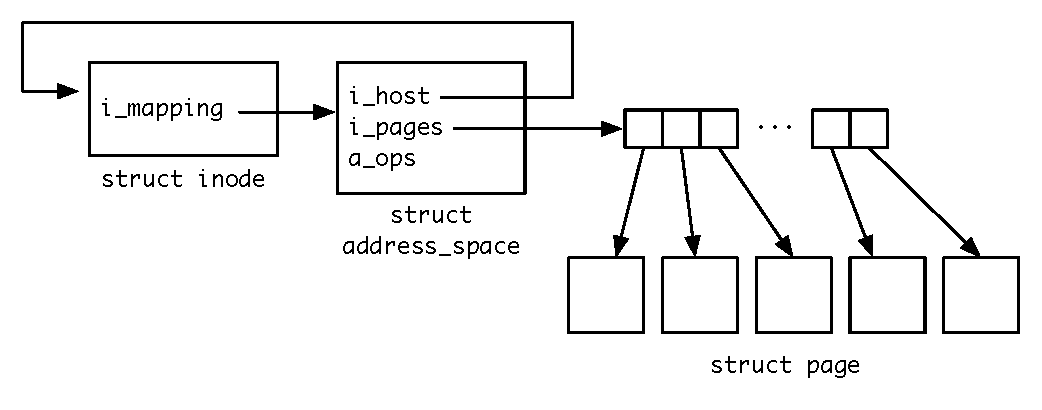
\includegraphics[scale=0.6]{figures/kstruct-inode-pages.pdf}
	\centering
	\caption{The Linux \cf{inode} which references data cached in memory}
	\label{fig:kstruct-inode-pages}
\end{figure}

\noindent
Although there may be multiple \cf{file} structures in memory representing different open instantiations of the same file from different processes, there will only be one \cf{inode} structure which is shared across all processes. File I/O and locking together with the internal operation of the inode cache will be described in section \cf{vfs-inode-cache}.

%%%%%%%%%%%%%%%%%%%%%%%%%%%%%%%%%%%%%%%%%%%%%%%%%%%%%%%%%%%%%%%%

\section{The Directory Cache}\label{kstruct-dcache}

Consider the simple command:

\begin{lstlisting}
$ [*\bfseries ls /home/spate/spfs/kern/spfs.ko*]
\end{lstlisting}

\noindent
To perform this operation, called \textit{pathname resolution}, the \cf{ls(1)} command calls the \cf{statx(2)} system call passing the pathname supplied as an argument. When parsing this pathname, the kernel has to process five different directories starting with "\cf{/}" and ending with "\cf{kern}".  As the path is being processed, it must validate that each directory in the path not only exists but that the caller has permission to access the directory. A permissions check is also performed on the base file. In this example, information about the regular file "\cf{spfs.ko}" is returned through a \cf{stat} structure. For an \cf{open(2)} call, the kernel finishes by setting up the structures described in the previous section and returning a file descriptor.

Each component of the pathname is represented by an \textit{inode} in a local filesystem or other entity over the network for filesystems such as NFS. Every time a call is made to the access a directory inside the filesystem, there can be many calls to read structures from disk which which is a time-consuming operation.  Accessing the same files happens frequently therefore minimizing disk access is imperative to improving the performance of the system. This is where the Linux \textit{dcache} (directory cache) comes into play. The dcache is a variation of the \textit{Directory Name Lookup Cache} (DNLC) which has been around for several decades now and was first introduced in BSD UNIX to solve the the \textit{pathname resolution} problem.

The Linux directory cache (simply called the \textit{dcache}) has the same goal as the original DNLC which is to provide a fast and efficient method of mapping any file name to a Linux inode regardless of the type of file. While resolving a pathname component for the first time, the kernel will ask the filesystem to lookup a filename within a specific directory. Once the filesystem locates this file, a reference to it can be stored in the dcache so that a subsequent lookup does not need to go to disk. Over the time, for frequently accessed files, the goal is to read from the dcache as much as possible. It is generally possible to get a dcache hit ratio of 80\% or higher.

%---------------------------------------------------------------------------------------------------------------------------------------------------------------------

\subsection{Introducing The \cf{dentry} Structure}

The main structure that underpins the dcache is the \cf{dentry} (directory entry). Dcache entries are searched using the parent directory dentry and a string for the file that is being searched for.

 \begin{table}[h]
\begin{tabular}{ll}
\parbox[l]{0.6in}{
\includegraphics[scale=0.8]{figures/src-xref.pdf}} & \parbox[l]{4in}{\small{The \cf{dentry} structure can be found in the \cf{include/linux/dcache.h} header file together with the global variable \cf{dentry\_hashtable} which references the dcache hash buckets.}}
\end{tabular}
\end{table}

 \noindent
 For each file that is present in the Linux dcache there is a dentry. After resolving the path "\cf{/mnt/file-a}", there are dentries in teh dcache for "\cf{/}", "\cf{mnt}" and "\cf{file-a}". Note that the dentry for "\cf{/}" will actually be present in the dcache from early in the boot process.
 
If the file "\cf{/mnt/file-a}" also has a hard link accessible via "\cf{/path-to-file-a}" and both entries are in the dcache, there will be two distinct dentries, one for "\cf{file-a}" and one for "\cf{path-to-file-a}".

Here are the basic set of \cf{dentry} fields. Others will be covered in later sections as the further details of the dcache are explored.

\begin{lstlisting}
struct [*\bfseries dentry*] {
    unsigned int                    d_flags;
    struct dentry                  *d_parent; 
    struct qstr                     d_name;
    unsigned char                   d_iname[DNAME_INLINE_LEN];    
    struct inode                   *d_inode;
    const struct dentry_operations *d_op;
    struct super_block             *d_sb;   
    struct hlist_bl_node            d_hash;
    struct list_head                d_lru; 
    struct list_head                d_child;    
    struct list_head                d_subdirs;  
    unsigned long                   d_time;  
    ...
}
\end{lstlisting}

\noindent
For the structure fields that are shown above, here is a general overview of their purpose:

\begin{itemize}
	\item \cf{d\_flags} -- there are a lot of flags. A few will be discussed below and others introduced as needed 
		throughout this section and in section \ref{vfs-dcache}.
	\item \cf{d\_parent} -- a pointer to the dentry for the parent directory.
	\item \cf{d\_iname} -- this field holds the name of the file if the size of the file name is less than 
		(\cf{DNAME\_INLINE\_LEN - 1}) bytes.
	\item \cf{d\_name} -- for small file names, the \cf{name} field within this \cf{qstr} structure will point to the \cf{d\_iname} field
		described above. For file names that are \cf{DNAME\_INLINE\_LEN} and longer, memory is allocated 
		and this field will point to the allocated memory where the file name is then stored.
	\item \cf{d\_inode} -- this field points to the Linux inode representing the underlying file. If the file doesn't exist, this
		field is set to \cf{NULL} and the dentry is known as a \textit{negative dentry}. Just as with files that exist, 
		negative dentries are useful to prevent repeated filesystem lookups.
	\item \cf{d\_op} -- filesystems can override / provide their own dcache functions that are called by the dcache when 
		performing specific operations. For local filesystems the dcache is expected to be a correct representation of 
		what's on disk but for network filesystems, a call may be needed to validate specific dentries since the cache
		may be out of date with respect to the server. This is because other clients may have made changes to a file
		making the dcache on this node out of date.
	\item \cf{d\_sb} -- the filesystem to which these dentries belong. This is particularly important during unmount
		and when pruning the dcache to reduce its memory footprint by getting easy access to all dentries for a 
		specific filesystem.
	\item \cf{d\_hash} -- the dcache itself is accessible through the \cf{dentry\_hashtable} global variable which is a large 
		collection of hash buckets. Which hash bucket to use is determined by calling the \cf{d\_hash()} function passing the 
		parent dentry and the file name. Each hash bucket can contain zero or more dentries linked through this field.
	\item \cf{d\_lru} -- all dentries that are not currently being accessed are collected on an LRU list linked through this 
		field. LRU lists are per filesystem and accessed through the \cf{s\_dentry\_lru} field of the \cf{super\_block} structure.
	\item \cf{d\_subdirs} /  \cf{d\_child} -- this field points to a list of dentries, one for each cached file within the directory 	
		referenced by this dentry. These child dentries are linked through \cf{d\_child}.
	\item \cf{d\_time} -- this field is only used by NFS and vboxfs to revalidate an entry after a specific time period has passed.
\end{itemize}

\noindent
The \cf{i\_dentry} field of the inode points to a list of dentries that reference this file. Note that there can be multiple links to the same file. For example:

\begin{lstlisting}
$ [*\bfseries touch /mnt/mydir/myfile*]
$ [*\bfseries ln /mnt/mydir/myfile link*]
\end{lstlisting}

\noindent
If the file were accessed using both paths there would be one inode for the actual file but two dentries, one for each file name. 

There are 35 different \cf{d\_flags} but not all flags will be covered in the book. A few are described below and other notable flags will be covered in section \ref{vfs-dcache} when the dcache implementation is described in more detail.

\begin{itemize}
	\item \cf{DCACHE\_MOUNTED} -- generally speaking, this flag is set on each dentry that has a filesystem mounted on 
		top of it.  Since Linux supports multiple filesystem namespaces, it is possible that the dentry may not be mounted 
		on in this namespace, therefore this flag is seen as a hint, not a guarantee.
	\item \cf{DCACHE\_LRU\_LIST} -- the dentry has no active holds and is therefore on the LRU list. It is quite possible
		that if the file is requested again, it will be found on this list before it is discarded.
	\item \cf{DCACHE\_REGULAR\_TYPE} -- this is a regular file. There are also flags for directories, symlinks 
		and special files.
	\item \cf{DCACHE\_NEED\_AUTOMOUNT} -- if the kernel needs to traverse into a directory for which this dentry flag
		is set, it has hit an auto-mount directory so an attempt is made to mount the remote filesystem before 
		pathname resolution can proceed.
	\item \cf{DCACHE\_REFERENCED} -- the dentry has recently been accessed and therefore it should not be discarded.
\end{itemize}

\noindent
There are seven flags that are set during dentry creation depending on whether the filesystem supports a list of \cf{dentry\_operations} (hanging off the \cf{s\_d\_op} field of the \cf{super\_block} structure). Most filesystems do not have such a list of operations but they are common for network filesystems. The flags can be found in \cf{dcache.h} by searching for \cf{DCACHE\_OP\_*}. For example, if the \cf{DCACHE\_OP\_COMPARE} flag is set when the kernel is looking up a file
in the dcache, a call is made into the filesystem to actually perform the comparison.

To show how the dentry structures are related, consider figure \ref{fig:kernel-pathname-tree} which shows a small file tree with a filesystem mounted on the directory \cf{mount-dir}.

\begin{figure}[h]
	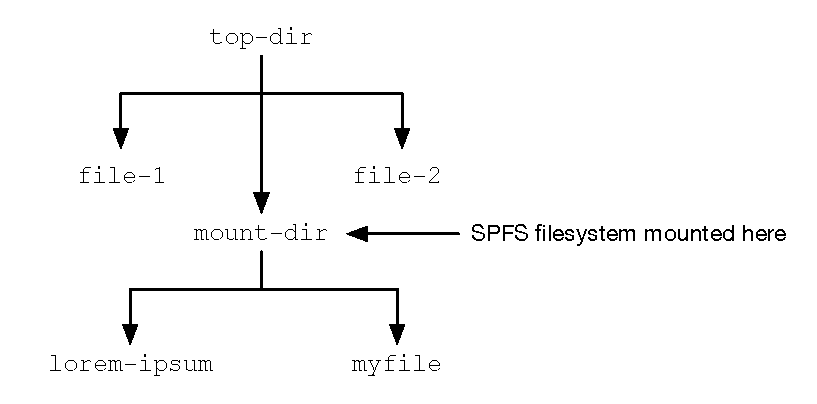
\includegraphics[scale=0.6]{figures/kernel-pathname-tree.pdf}
	\centering
	\caption{A simple example file hierarchy}
	\label{fig:kernel-pathname-tree}
\end{figure}

For this particular tree, if we assume that all dentries are in the dcache, they are connected as shown in figure \ref{fig:kernel-pathname-dentries}. The figure shows the connection between the parent and child dentries through the \cf{d\_parent}, \cf{d\_subdirs} and \cf{d\_child} fields. Notice that there is no direct connection between the base filesystem and the filesystem that is mounted on \cf{mount-dir}. However, the \cf{DCACHE\_MOUNTED} mounted flag will generally be set on the dentry for \cf{mount-dir} indicating that the directory has been mounted on. \textbf{This isn't always true in the case of namespace which will be covered later.}

\begin{figure}[h]
	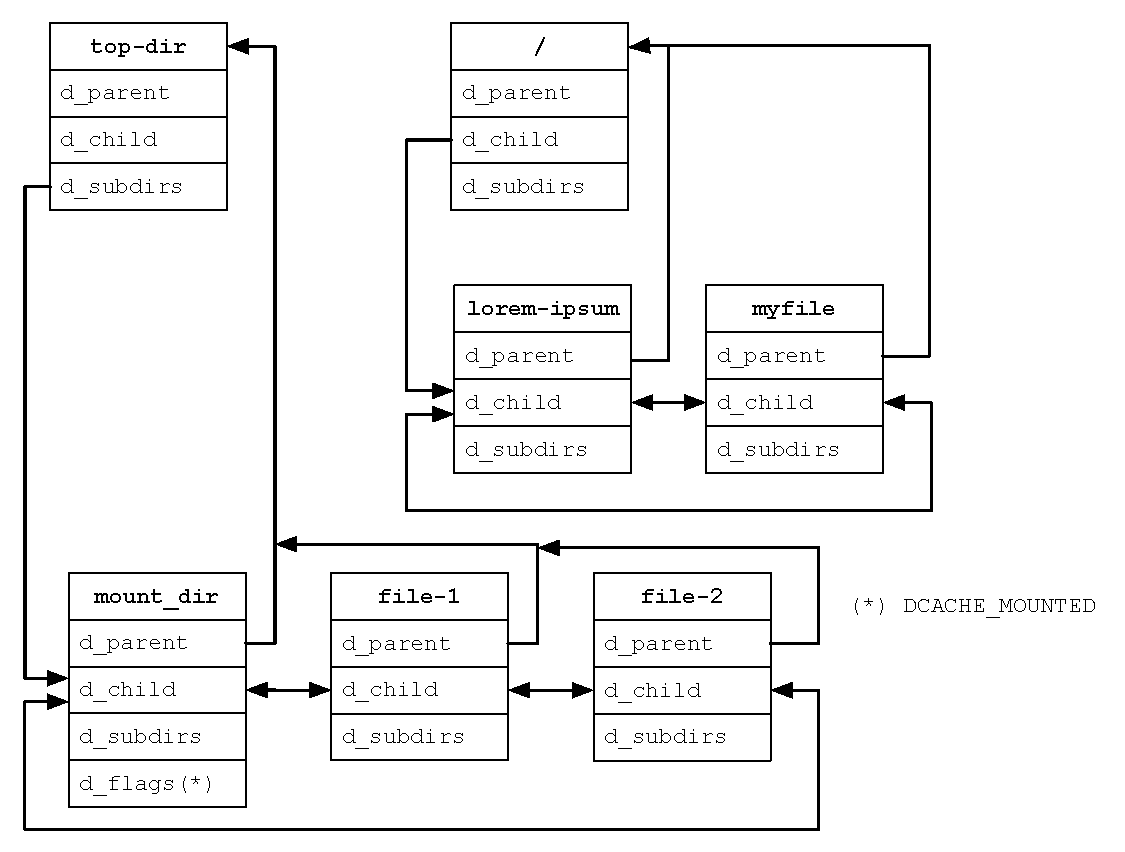
\includegraphics[scale=0.6]{figures/kernel-pathname-dentries.pdf}
	\centering
	\caption{dentries for the example file hiearchy}
	\label{fig:kernel-pathname-dentries}
\end{figure}

%------------------------------------------------------------------------------------------------------------------------------------------------------------------------

\subsection{Dcache Hash Buckets}

The Linux dcache is basically a large list of hash buckets and is accessed through the glocal \cf{dentry\_hashtable} variable:

\begin{lstlisting}
static struct hlist_bl_head *dentry_hashtable
\end{lstlisting}

\noindent
A simple example of how \cf{dentry\_hashtable} references the hash buckets is shown in figure \ref{fig:kernel-dentry-hashtable}. Each dentry in the cache is hashed using the dentry of its parent and the file name. To see if a file name is present in the cache, the kernel hashes to get the correct hash bucket then walks the appropriate list to look for the entry that it's searching for. Hash lists are generally fairly short, again helping with performance.


\begin{figure}[h]
	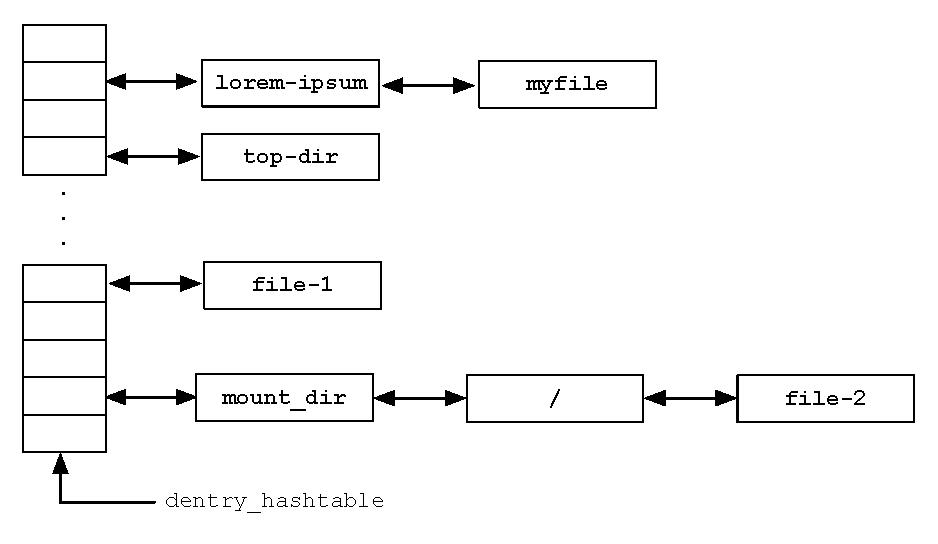
\includegraphics[scale=0.6]{figures/kernel-dentry_hashtable.pdf}
	\centering
	\caption{The dcache headed by \cf{dentry\_hashtable}}
	\label{fig:kernel-dentry-hashtable}
\end{figure}

Each element in the hash table is a pointer to a list of dentries that hash to the same value. The function \cf{d\_hash()} calculates the hash and thus gives access to the right hash bucket.

\begin{lstlisting}
static inline struct hlist_bl_head *
[*\bfseries d\_hash(unsigned int hash)*]
{
    return [*\bfseries dentry\_hashtable*] + (hash >> d_hash_shift);
}
\end{lstlisting}

\noindent
There is quite a lot of code behind hashing to locate the correct bucket. Section \ref{dcache-hash} covers the process in more detail. \textbf{XXX -- not sure it does but come back to this}.

%------------------------------------------------------------------------------------------------------------------------------------------------------------------------

\subsection{KGDB -- Analyzing The Dcache}

\textbf{XXX -- there is something wrong here. One entry in the left column and others the right column. Need to fix}

This example shows how to dump out part of the dcache hash table and view some of the dentries. The dcache is accessed through \cf{dentry\_hashtable} and each hash bucket is of the following type:

\begin{lstlisting}
struct [*\bfseries hlist\_bl\_node*] {
    struct hlist_bl_node *next, **pprev;
};
\end{lstlisting}

\noindent
Starting at \cf{dentry\_hashtable}, each bucket occupies two addresses (forward and back pointers). Here we display 24 addresses:

\begin{lstlisting}
(gdb) [*\bfseries x/24a dentry\_hashtable*]
0xffff88817b800000:    0x0                0x0     
0xffff88817b800010:    0x0                0xffff888103132248
0xffff88817b800020:    0x0                0x0
0xffff88817b800030:    0x0                0x0 
0xffff88817b800040:    0x0                0x0
0xffff88817b800050:    0x0                0x0 
0xffff88817b800060:    0x0                0x0
0xffff88817b800070:    0x0                0x0
0xffff88817b800080:    0x0                0x0
0xffff88817b800090:    0xffff888101a816c8 0x0
0xffff88817b8000a0:    0x0                0x0
0xffff88817b8000b0:    0x0                0xffff8881013a6788
\end{lstlisting}

\noindent
The first thing to notice and especially if you dump more addresses is that most buckets are empty. Taking the first address displayed, we need to call \cf{container\_of()} to get to the dentry since this list goes through the \cf{d\_hash} field of the dentry structure.

\begin{lstlisting}
(gdb) [*\bfseries set \$de = \$container\_of(0xffff888103132248, \textbackslash*]
                                      [*\bfseries "struct dentry", "d\_hash")*]
\end{lstlisting}

\noindent
Now let's display the name of the file and the contents of the \cf{d\_hash} field:         

\begin{lstlisting}
(gdb) [*\bfseries p \$de->d\_iname*]
$213 = "warnings", '\000' <repeats 23 times>
(gdb) [*\bfseries p \$de->d\_hash*]
$216 = {
  next = 0x0 <fixed_percpu_data>,
  pprev = 0xffff88817b800018
}
\end{lstlisting}

\noindent
In this example, the \cf{next} field is NULL and the \cf{pprev} field points back to the head of the hash bucket itself. Therefore this is the only dentry in this bucket. An interesting point is the dentry pointer at address \cf{0xffff88817b800090} which is also a single dentry. Why one entry is accessible through the \cf{next} field of a \cf{hlist\_bl\_node} structure and another is through the \cf{pprev} field is a bit of a mystery. \textbf{XXX -- come back here if time allows. I may have something wrong?}

%------------------------------------------------------------------------------------------------------------------------------------------------------------------------

\subsection{Overriding / Supporting Dcache Operations}

There is a structure defining a list of \cf{dentry\_operations} that some filesystems support. Most filesystems don't do anything in this regard as entries in the dcache are expected to be an accurate representation of what's on disk. The kernel and local filesystems work in conjunction to make sure that the dcache is accurate.  However, this is not always the case with network filesystems such as NFS since other clients may perform operations that result in changes on the server which have not yet been reflected on this client potentially causing invalid dentries. Another example is the FAT filesystem which is not case sensitive so provides a \cf{d\_compare()} function to implement the comparison operations.

The list of operations are for this structure are:

\begin{lstlisting}
struct [*\bfseries dentry\_operations*] {
    int    (*d_revalidate)(struct dentry *, unsigned int);
    int    (*d_weak_revalidate)(struct dentry *, unsigned int);
    int    (*d_hash)(const struct dentry *, struct qstr *);
    int    (*d_compare)(const struct dentry *,
                        unsigned int, const char *, 
                        const struct qstr *);
    int    (*d_delete)(const struct dentry *);
    int    (*d_init)(struct dentry *);
    void   (*d_release)(struct dentry *);
    void   (*d_prune)(struct dentry *);
    void   (*d_iput)(struct dentry *, struct inode *);
    char * (*d_dname)(struct dentry *, char *, int);
    struct vfsmount *(*d_automount)(struct path *);
    int    (*d_manage)(const struct path *, bool);
    struct dentry *(*d_real)(struct dentry *, 
                             const struct inode *);
}
\end{lstlisting}

\noindent
This structure and functions will further be discussed in section \ref{vfs-dcache}. \textbf{XXX -- It will?}

%%%%%%%%%%%%%%%%%%%%%%%%%%%%%%%%%%%%%%%%%%%%%%%%%%%%%%%%%%%%%%

\section{The Inode Cache}\label{kstruct-inodes}

In UNIX, a file stored on a physical disk was traditionally been referenced by a structure stored on disk called an \textit{inode} which contained information about all parts of the file including owner, group, size of the file and pointers to the actual data. When a file was accessed by the kernel, the filesystem would bring the inode into memory and parts of it were copied into an \textit{in-core inode}. This is somewhat confusing since it didn't take long before there were multiple filesystems and some filesystems did not have inodes (NFS being the perfect example). Although both inode structures reference the same file, their purposes are different. The in-core inode is generic across all filesystems and has no built-in knowledge of the on-disk structure whereas the disk inode describes how the file's data and meta-data are stored on disk and is specific to the filesystem on which it belongs. With SunOS and SVR4 UNIX, the in-core structure was renamed and became a \cf{vnode} structure to help distinguish between the two different entities which could often be very different. Add to that, network filesystems don't have inodes on the client and their internal structures were represented by different structures (\textit{snodes} for NFS and \textit{rnodes} for RFS). Linux kept the original UNIX nomenclature and has inodes for both in-core and on-disk structures. Of course Linux filesystems are free to implement whatever mechanisms they want for representing files. 

Accessing a file for the first time can be a time-consuming operation and involve several disk I/Os as described above in section \ref{kstruct-dcache}. In addition to the dcache, Linux maintains an in-core cache of recently accessed inodes. All cached inodes are associated with the mounted filesystem to which they belong so are easy to access when performing operations such as syncing data or unmounting a filesystem.

Inodes are shared between processes such that if two process have the same file open, there will only be one inode. Per-process information such as the file offset are process-specific and are held in the \cf{file} structure as described earlier. 

\begin{table}[h]
\begin{tabular}{ll}
\parbox[l]{0.6in}{
\includegraphics[scale=0.8]{figures/src-xref.pdf}} & \parbox[l]{4in}{\small{Linux inodes are represented by the \cf{inode} structure which can be found in \cf{include/linux/fs.h}}}
\end{tabular}
\end{table}


\noindent
A subset of the fields of the inode are shown below. Several are self-explanatory and are returned when calling the \cf{stat(2)} system call on a file.

\begin{lstlisting}
struct inode {                     
    umode_t                        i_mode;
    kuid_t                         i_uid;
    kgid_t                         i_gid;
    unsigned int                   i_flags;
    const struct inode_operations *i_op;
    struct super_block            *i_sb;
    struct address_space          *i_mapping;
    unsigned long                  i_ino;
    const unsigned int             i_nlink;
    dev_t                          i_rdev;
    loff_t                         i_size;
    struct timespec64              i_atime;
    struct timespec64              i_mtime;
    struct timespec64              i_ctime;
    unsigned short                 i_bytes;
    blkcnt_t                       i_blocks;
    struct address_space           i_data;
    void                          *i_private;
} 
\end{lstlisting}

\noindent
Throughout the book the term \textit{Linux inode} or \textit{in-core inode} will be used in order to distinguish these inodes from the disk-based inodes implemented by various filesystems. The fields of the \cf{inode} structure that require explanation at this point are:

\begin{itemize}
	\item \cf{i\_ino} -- the inode number which is unique across the filesystem to which this file resides.
	\item \cf{i\_nlink} -- the number of links to this file. For regular files this will be "1" when the file is created and is
		incremented when a hard link is created for which the file name references this file.
	\item \cf{i\_op} -- a list of operations that can be performed on this file. The operations are set by
		the filesystem when the file is opened and are generally applicable to directories. Operations include
		lookup (locate a file in the directory), file and directory creation and file removal. 
	\item \cf{i\_sb} -- a pointer to the \cf{super\_block} structure representing the mounted filesystem 
		to which this file belongs. This will be described in section \ref{superblock}.
	\item \cf{i\_mapping} -- for regular files, this points to an \cf{address\_space} structure which is used
		to reference pages in memory through which file I/O occurs. These pages contain cached data and can also
		contain data that needs to be written to disk. This will be explored in section \ref{page-cache}.
	\item \cf{i\_private} -- the \cf{inode} structure represents the in-core instantiation of the file. When files are accessed, the 
		underlying filesystem will read in its own inode (or other structure depending on the type of filesystem) and may
		cache parts of that structure in memory allocated by the filesystem. This field can point to a per-file private 
		data structure. However, most Linux filesystems no longer use this field and have the Linux inode embedded 
		within the filesystem inode and use the \cf{container\_of()} macro to move from the Linux inode structure to 
		the filesystem data. This will be described in section \ref{container-of} and examples are shown throughout the book.
\end{itemize}

\noindent
There are various lists of inodes associated with each mounted filesystem. A particular inode can be on one of the following lists:

\begin{itemize}
	\item \cf{i\_hash} -- hash list used for locating inodes quickly using the inode number. 
	\item \cf{i\_lru} -- a list of least recently used inodes.
	\item \cf{i\_io\_list} -- TBD	
	\item \cf{i\_sb\_list} -- a linked list of all inodes associated with the mounted filesystem to which this file belongs.
	\item \cf{i\_wb\_list} -- TBD
	\item \cf{i\_dentry} -- a list of dentries that are referencing this file. 
	\item \cf{i\_rcu} -- TBD
\end{itemize}

\noindent
TBD

There is no longer a single inode cache. Each filesystem has its own cache to which inodes are added when allocated. Each mounted filesystem has the following inode-related fields inside the \cf{super\_block} structure:

\begin{lstlisting}
struct list_lru     s_inode_lru;
struct list_head    s_inodes;       /* all inodes */
struct list_head    s_inodes_wb;    /* writeback inodes */
\end{lstlisting}

\noindent
Typing things together, figure \ref{fig:kstruct-inodes} shows inodes hanging off the \cf{super\_block} structure referenced by the \cf{s\_inodes} field.

\begin{figure}[h]
	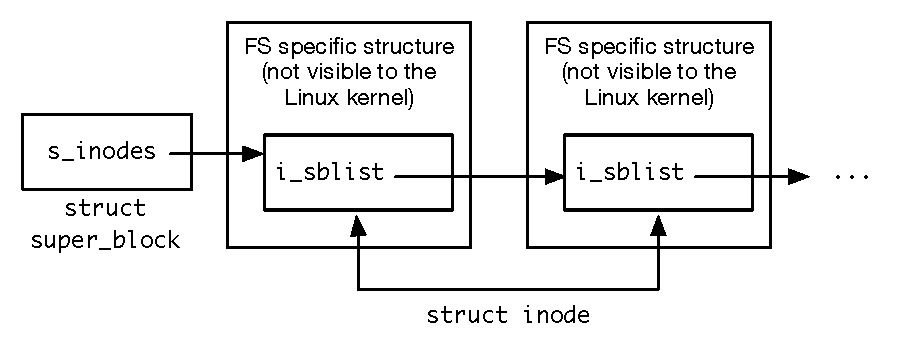
\includegraphics[scale=0.6]{figures/kstruct-inodes.pdf}
	\centering
	\caption{The inode cache for each mounted filesystem}
	\label{fig:kstruct-inodes}
\end{figure}

\noindent
This list makes it easy to locate all filesystem inodes which is particularly important when unmounting the filesystem.

%---------------------------------------------------------------------------------------------------------------------------------------------------------------------

\subsection{KGDB -- Analyzing Per-File Kernel Structures}\label{fd-analyze}

In this demonstration, we will analyze a process that opens a file, keeps the file open allowing us to show the kernel structures from the \cf{task\_struct} through to the inode where we can verify the inode number. The goal is to follow the links shown in figure \ref{fig:per-file-kernel-structures}.

Below is a very simple program which opens a file and then pauses indefinitely (waiting for a signal). This allows us to search to files open by this process. We call the binary something obvious / unique to make it easy to search for, in this case "\cf{open-spate}". The inode number associated with this file is also shown. An inode number is guaranteed to be unique within a filesystem although not across all filesystems. In this case the inode number is 407688.

\begin{lstlisting}
int
main()
{
    int fd = open("lorem-ipsum", O_RDONLY);
    pause();
}
\end{lstlisting}

\noindent

\begin{lstlisting}
$ [*\bfseries ls -li lorem-ipsum*]
[*\bfseries 407688*] -rw-r--r-- 1 spate spate 2972 Dec  4 15:43 lorem-ipsum
\end{lstlisting}

\noindent
Once \cf{gdb} is running, several \cf{gdb} commands will be executed to get us through the structures to locate the inode and verify that we have the right inode number. As we walk through \cf{gdb} sessions, I'm going to assume that many readers may not be very familiar with the workings of \cf{gdb} so will be somewhat more elaborate in showing the stages of moving from one structure to the next. For example, you don't need to use convenience variables but they certainly help a lot. A convenience variable is simply a variable that you can assign a value to. Once we find the \cf{file} structure, we can assign the address to a variable called \cf{file} for easier reference in future.

Now assuming the program above is running, we can use one of the Linux helper functions to locate the \cf{task\_struct} for the running process. The \cf{pipe} command is very useful in this instance. We store the address displayed in the variable \cf{ts}.

\begin{lstlisting}
(gdb) [*\bfseries pipe lx-ps | grep spate*]
0xffff0000f34890c0 1213  open-spate

(gdb) [*\bfseries set \$ts = (struct task\_struct *)0xffff0000f34890c0*]
\end{lstlisting}

\noindent
The next step is to display the \cf{files} field and assign it to \cf{files}. Note that we use \cf{\$2} here and could actually use \cf{\$2} rather than assign it to a convenience variable. You can use either option.

\begin{lstlisting}
(gdb) [*\bfseries p \$ts->files*]
$2 = (struct files_struct *) 0xffff0000f3aa2100

(gdb) [*\bfseries set \$files = \$2*]
\end{lstlisting}

\noindent
Next we display the whole \cf{files\_struct} structure. 

\begin{lstlisting}
(gdb) [*\bfseries p *\$files->fdt*]
$22 = {
  max_fds = 256,
  fd = 0xffff0000f38c3000,
  close_on_exec = 0xffff0000ec53efa0,
  open_fds = 0xffff0000ec53ef80,
  full_fds_bits = 0xffff0000ec53efc0,
  rcu = {
    next = 0x0,
    func = 0x0
  }
}
\end{lstlisting}

\noindent
The \cf{open\_fds} field points to a bitmap of which file descriptors have been allocated. Below, you can see mostly \cf{0}s followed by 4 \cf{1}s representing allocated file descriptors 0, 1, 2 and 3. The \cf{fd} field of \cf{files\_struct} contains an array of file descriptors.  We dump the contents of memory to display the first 4 addresses:

\begin{lstlisting}
(gdb) [*\bfseries x/t 0xffff0000ec53ef80*]
0xffff0000cacad200:	000000000000...00000000000000000001111
(gdb) [*\bfseries x/4a \$files->fdt.fd*]
0xffff0000f38c3000:	0xffff0000c1fb6f00   0xffff0000c1fb6f00
0xffff0000f38c3010:	0xffff0000c1fb6f00   0xffff0000ca4f7500
\end{lstlisting}

\noindent
The \cf{fd} field points to an array of pointers to \cf{file} structures, one per file descriptor. The reason for displaying 4 addresses is that these addresses are the first 4 elements of the array and there is one for each of the 4 open files for this process (recall that 0, 1 and 2 are for \cf{stdin}, \cf{stdout} and \cf{stderr}). The last address should point to the \cf{file} structure for our open file \cf{lorem-ipsum}. 

Next we store its value and print out the \cf{file} structure (I've omitted most fields). You can see the file position (\cf{f\_pos}) which is \cf{0} since the file has just been opened but no reads or writes have taken place.

\begin{lstlisting}
(gdb) [*\bfseries set \$file = (struct file *)0xffff0000ca4f7500*]
(gdb) [*\bfseries p *\$file*]
  f_path = {
    mnt = 0xffff0000c08352e0,
    dentry = 0xffff0000cfc92840
  f_inode = 0xffff0000cfcf6c40,
  f_op = 0xffff8000092c5e00 <ext4_file_operations>,
  f_flags = 131072,
  f_mode = 1212842013,
  f_pos = 0,
  f_cred = 0xffff0000f4deb540,
  f_mapping = 0xffff0000cfcf6db8,
}
\end{lstlisting}

\noindent
You can also see a reference to the dentry for this file (we will cover dentries soon) but for now, we can just display the part of the \cf{dentry} structure to confirm the file name:

\begin{lstlisting}
(gdb) [*\bfseries p \$file->f\_path.dentry->d\_name.name*]
$32 = (const unsigned char *) 0xffff0000cfc92878 "lorem-ipsum"
\end{lstlisting}

\noindent
Finally, we save the address of the \cf{inode} structure and display the inode number which matches what the \cf{ls(1)} command showed above.

\begin{lstlisting}
(gdb) [*\bfseries set \$ip = (struct inode *)0xffff0000cfcf6c40*]
(gdb) [*\bfseries p \$ip->i\_ino*]
$26 = 407688
\end{lstlisting}

\noindent
There is a lot to take in here so I suggest that you try this example yourself. Perhaps open more files and look for each one or explore the \cf{file} structure for \cf{stdin}.

%----------------------------------------------------------------------------------------------------------------------------------------------------------------

\subsection{Analyzing Per-File Kernel Structures Using \cf{crash}}

Here is the same analysis as shown in the previous section but this time using the \cf{crash(1)} command. All of the steps above are repeated but this time using \cf{crash} commands on a live system (note different addresses due to running both sessions at different times).

The first step is to run the \cf{ps} command and search for the running process:

\begin{lstlisting}
crash> [*\bfseries ps | grep spate*]
   7703   5214   3  ffff5a09d824af40 IN 0.0 2056 968 open-spate
\end{lstlisting}

\noindent
The \cf{task\_struct} structure address is shown. Here we look for the \cf{files} field. You can also run "\cf{struct task\_struct}" to achieve the same result but usually just typing the structure name by itself will suffice.

\begin{lstlisting}
crash> [*\bfseries task ffff5a09d824af40 | grep files*]
  files = 0xffff5a09c08f7c80,
\end{lstlisting}

\noindent
The next step is to locate the file table and from there, get the pointer to the file descriptor array:

\begin{lstlisting}
crash> [*\bfseries files\_struct 0xffff5a09c08f7c80 | grep "fdt ="*]
  fdt = 0xffff5a09d8814800,
  fdtab = {

crash> [*\bfseries fdtable 0xffff5a09d8814800 | grep "fd ="*]
  fd = 0xffff5a09d4292800,
\end{lstlisting}

\noindent
As with the previous example, we dump memory and see \cf{file} structure pointers for the first four file descriptors. From here we can show the filename through its \cf{dentry} and locate the \cf{inode} structure to get the inode number.

\begin{lstlisting}
crash> [*\bfseries rd 0xffff5a09d4292800 4*]
ffff5a09d4292800:  ffff5a09d97a1200 ffff5a09d97a1200 
ffff5a09d4292810:  ffff5a09d97a1200 ffff5a09b2bf7200  

crash> [*\bfseries file ffff5a09b2bf7200 | grep dentry*]
    dentry = 0xffff5a09b6de2f00

crash> [*\bfseries dentry 0xffff5a09b6de2f00 | grep name*]
  d_name = {
    name = 0xffff5a09b6de2f38 "lorem-ipsum"
  d_iname = "lorem-ipsum\000\000\000\0...0\000\000\000\000",

crash> [*\bfseries file ffff5a09b2bf7200 | grep inode*]
  f_inode = 0xffff5a095f42a140,

crash> [*\bfseries inode 0xffff5a095f42a140 | grep i\_ino*]
  i_ino = 407688,
\end{lstlisting}

\noindent
Generally speaking, with \cf{gdb} integrated into \cf{crash} you can achieve the same results with both debuggers and it's certainly easier to set up \cf{crash} with only one system being needed. But when it comes to setting breakpoints, you will need \cf{gdb}. Chapter \ref{{debugging}} will show how to set breakpoints in the kernel with \cf{gdb} / \cf{kgdb}.

\subsection{KGDB --- Multiple dentries Per Single File}

The \cf{inode} structure is shared between different processes access the same file but can also be accessed by two different open files in the same process. In this example we show a case where we have a file with two hard links as follows:

\begin{lstlisting}
# [*\bfseries ls -li*]
total 1
4 -rw-r--r-- 2 root root 2972 Jan 23 21:07 hard-link
4 -rw-r--r-- 2 root root 2972 Jan 23 21:07 lorem-ipsum
\end{lstlisting}

\noindent
You can see that both files have an inode number of 4. Both files will be opened by the following program which then pauses waiting on a signal giving us unlimited time to analyze the kernel structures:

\begin{lstlisting}
    int fd1 = open("lorem-ipsum", O_RDONLY);
    int fd2 = open("hard-link", O_RDONLY);
    pause();
\end{lstlisting}

\noindent
In \cf{gdb} we go through a similar sequence as the previous example to get to the file descriptor array to locate the \cf{file} structures corresponding to file descriptors 4 and 5.

\begin{lstlisting}
(gdb) [*\bfseries p \$ts->files->fdt->fd*]
$118 = (struct file **) 0xffff0000e42a7000
(gdb) [*\bfseries x/5a 0xffff0000e42a7000*]
0xffff0000e42a7000:    0xffff0000f477a400    0xffff0000f477a400
0xffff0000e42a7010:    0xffff0000f477a400    0xffff0000d1050000
0xffff0000e42a7020:    0xffff0000d1050100
(gdb) [*\bfseries set \$file1 = (struct file *)0xffff0000d1050000*]
(gdb) [*\bfseries set \$file2 = (struct file *)0xffff0000d1050100*]
\end{lstlisting}

\noindent
From here, we print out the inode structures which match as expected. We also show the dentries for each open instance showing the two filenames.

\begin{lstlisting}
(gdb) [*\bfseries p \$file1->f\_inode*]
$119 = (struct inode *) 0xffff0000f18a9780
(gdb) [*\bfseries p \$file2->f\_inode*]
$120 = (struct inode *) 0xffff0000f18a9780
(gdb) [*\bfseries p \$file1->f\_path->dentry->d\_name.name*]
$121 = (const unsigned char *) 0xffff0000d29573f8 "lorem-ipsum"
(gdb) [*\bfseries p \$file2->f\_path->dentry->d\_name.name*]
$122 = (const unsigned char *) 0xffff0000d29397b8 "hard-link"
(gdb) [*\bfseries p \$file1->f\_inode->i\_ino*]
$2 = 4
(gdb) [*\bfseries p \$file1->f\_inode->i\_private*]
$4 = (void *) 0x8300000002
\end{lstlisting}

\noindent
We also show that it's inode number 4. This time we have a private data structure that's held by the filesystem. This was how the SPFS filesystem was originally implemented to map the Linux inode to the SPFS inode. See \ref{disk-fs} for more details.

\section{The Buffer Cache}

In earlier versions of UNIX up to around SVR3, all data that was read from, or written to disk, went through the \textit{buffer cache}. At the heart of the buffer cache was a structure (\cf{struct buf}) and a set of routes such as \cf{getblk()}, \cf{bread()}, \cf{bwrite()} and \cf{brelse()} to get a block for a specified device, read or write a block and then release the block once the caller had finished with it.

Everything changed in the 1980s with the introduction of a new virtual memory (VM) architecture in Sun's SunOS which was also replicated in SVR4 UNIX. File I/O was taken out of the buffer cache and integrated into the new VM subsystem where filesystems were called with sets of pages which needed to be read or written. This hybrid buffer/page cache model is the approach that Linux has followed in that file I/O does not go through the buffer cache. There are still many things that the filesystem needs to read/write that are not regular file contents namely directory entries, inodes, extended attributes, symlinks and so on. And these structures and therefore corresponding blocks on disk, are likely to be read repeatedly. As discussed already, reading and writing data from/to disk repeatedly is slow and this results in the need for another cache, the \textit{buffer cache}.

The main data structure used by the buffer cache is the \cf{buffer\_head} structure (akin to the old UNIX \cf{buf} structure). 

\begin{table}[h]
\begin{tabular}{ll}
\parbox[l]{0.6in}{
\includegraphics[scale=0.8]{figures/src-xref.pdf}} & \parbox[l]{4in}{\small{\cf{include/linux/buffer\_head.h} contains the definition of the \cf{buffer\_head} structure}}
\end{tabular}
\end{table}

\noindent
The main fields in this structure are:

\begin{itemize}
	\item \cf{b\_data} -- a pointer to a memory area where the data is or will be located.
	\item \cf{b\_size} -- the size of the buffer.
	\item \cf{b\_bdev} -- the block device to which the buffer belongs.
	\item \cf{b\_blocknr} -- the block number on the device to which this buffer refers to.
	\item \cf{b\_state} -- the status of the buffer including \cf{BH\_Uptodate} (contents are valid) and 
		\cf{BH\_Dirty} (buffer needs writing to disk).
	\item \cf{b\_count} -- the buffer's reference count. Before a buffer is returned to a caller, this field is incremented. 
		It is subsequently decremented when the caller releases the buffer (see \cf{brelse()} below.
\end{itemize}

\noindent
Here are some important functions:

\begin{itemize}
	\item \cf{\_\_bread()} -- reads a block using the specified block number and given size. If the read is successful, 
		a pointer to the  \cf{buffer\_head} structure, otherwise \cf{NULL} is returned.
	\item \cf{sb\_bread()} -- this is the same as \cf{\_\_bread()} but the size of the read block 
		is taken from the \cf{super\_block} structure in addition to the device from which the read will be performed.
	\item \cf{mark\_buffer\_dirty()} -- marks the buffer as dirty (sets the \cf{BH\_Dirty} bit). The buffer will be written 
		to the disk at a later time (from time to time the bdflush kernel thread wakes up and writes the buffers 
		to disk). \textbf{XXX -- need to check that this is still the case}
	\item \cf{brelse()} --  frees up the memory used by the buffer, after the buffer has been written to disk 
		(if needed.
	\item \cf{map\_bh()} -- \textbf{associate the buffer-head with the corresponding sector. very poor descriptions out there.
		I use in sp\_get\_block() so find a better description.}
\end{itemize}

\noindent
Although jumping ahead a little, here is an example of how the buffer cache is used. For our disk-based filesystem SPFS (section \ref{disk-fs}), we need to read in the \textit{superblock} from block 0 on disk to access basic information about the filesystem that is being mounted. The kernel calls into a filesystem-supplied function as part of mount processing. Here is a fragment of the code in this function:

\begin{lstlisting}
spfs_fill_super(struct super_block *sb, void *data, int silent)
{
    struct sp_superblock    *spfs_sb;
    struct buffer_head      *bh;

    bh = [*\bfseries sb\_bread*](sb, 0);
    if (!bh) {
        goto out;
    }
    spfs_sb = (struct sp_superblock *)bh->b_data;
\end{lstlisting}

\noindent
When the filesystem is initialized, an internal \cf{super\_block} structure is allocated. One of the fields of this structure is the device on which the filesystem resides and another is the block size used for this filesystem/device. The SPFS \cf{spfs\_fill\_super()} function is called as part of mount processing. It calls \cf{sb\_read()} to read in block 0 which is where the SPFS superblock is held. It fits in one block regardless of the block size.

Filesystems will generally call \cf{sb\_bread()} when reading blocks from disk (\textbf{what about writing?}). You will see a few exceptions in the individual files (run "\cf{grep \_\_bread fs/*}" at the top of the kernel source tree) to see examples. One specific example is ext4 which states above the function \cf{\_\_ext4\_sb\_bread\_gfp()}:

\begin{quote}
\textit{Currently with sb\_bread it's impossible to distinguish between ENOMEM and EIO situations (since both result in a NULL return.}
\end{quote}

\noindent
Instead of calling \cf{sb\_bread()}, ext4 calls \cf{sb\_getblk\_gfp()}. If it returns \cf{NULL}, ext4 can interpret that as an \cf{ENOMEM} condition.

\subsection{Buffer Cache Size / Usage}

The amount of space currently used by the buffer cache can be seen through \cf{/proc}:

\begin{lstlisting}
$ [*\bfseries grep Buffers /proc/meminfo*]
Buffers:          326920 kB
\end{lstlisting}

\noindent
To see this value change, simply run the command "\cf{find /}" which will result in a lot of calls in to the different mounted filesystem to read inodes and directory entries. Let it run for a while and then stop it. Look inside \cf{/proc/meminfo} again and you will likely see the value increase.

But how much space will be used? That depends on how much memory is available and what type of activity is being performed. If there is a lot of I/O that requires the buffer cache, the amount of space will increase. If memory is required for other purposes, it will be reclaimed and reused. Operating systems used to be much more restrictive on the amount of memory available for different caches. But some caches could be underutilized resulting in wasted memory. If there is a lot of activity around file meta-data, it makes sense to let the buffer cache grow. If the system is doing a lot of I/O, utilize the page cache. Memory can always be reclaimed to serve the needs of what is happening at any moment in time.

\textbf{XXX---can be reclaimed but how often is that useful? Section in next chapter that covers the buffer cache in more detail?}

\subsection{Flushing Buffers}

When dirty buffers are released, the data is not immediately written to disk. If there is no need to write it straightaway, why do so? It could be perfectly valid for a caller to request the same buffer again, update it and release it once more. Why issue two writes instead of one? When to write dirty buffers and how often has been a hotly debated topic for a very long time and in Linux, this is no exception.

In the early days of Linux, there was \cf{bdflush}, a user process that called into the kernel to periodically sync buffers. User processes can be killed so this was replaced by a kernel thread but that also ran into issues on larger systems. This single thread would become a bottleneck. The next step was to replace \cf{bdflush} with multiple threads (called \cf{pdflush}), one per physical drive. The \cf{pdflush} threads were eventually removed and replaced with a more elaborate scheme.

\textbf{XXX---come back when doing the performance chapter}

%%%%%%%%%%%%%%%%%%%%%%%%%%%%%%%%%%%%%%%%%%%%%%%%%%%%%%%%%%%%%%%

\section{The Page Cache}\label{page-cache}

% https://www.kernel.org/doc/html/latest/filesystems/vfs.html

% https://stackoverflow.com/questions/32047144/whats-the-difference-between-inode-i-data-and-inode-i-mapping

As described above, meta data data is read from / written to disk through the buffer cache. All file data is read from / written to the \textit{page cache}. Figure \ref{fig:address-space} shows how in-memory pages are associated with an individual inode. As with most data on disk, it's assumed that the data will be accessed repeatedly so caching it in memory to reduce the number of disk accesses is paramount to having a high-performing system. \textbf{XXX---check this figure is correct once kgdb running}

\begin{figure}[h]
	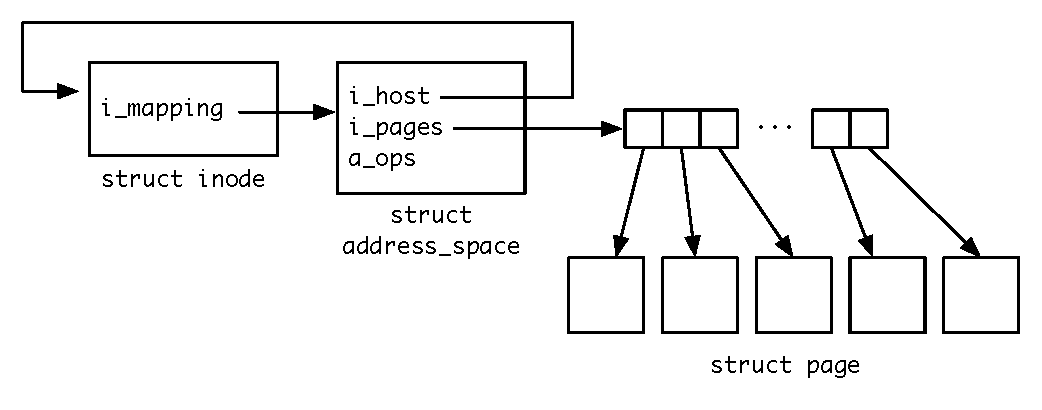
\includegraphics[scale=0.6]{figures/address-space.pdf}
	\centering
	\caption{Relationship between inodes and the page cache}
	\label{fig:address-space}
\end{figure}

\begin{table}[h]
\begin{tabular}{ll}
\parbox[l]{0.6in}{
\includegraphics[scale=0.8]{figures/src-xref.pdf}} & \parbox[l]{4in}{\small{The \cf{address\_space} structure is defined in \cf{include/linux/fs.h}}}
\end{tabular}
\end{table}

\noindent
A few of the fields of the \cf{address\_space} structure are shown below:

\begin{lstlisting}
struct address_space {
    struct inode                          *host;
    struct xarray                          i_pages;
    unsigned long                          nrpages;
    const struct address_space_operations *a_ops;
    unsigned long                          flags;
    ...
}
\end{lstlisting}

\noindent
All pages that are currently cached in memory are referenced through the \cf{i\_pages} field. An \cf{xarray} structure XXX

% https://lwn.net/Articles/745073/

% https://stackoverflow.com/questions/31966298/can-we-access-memory-through-a-struct-page-structure - need to call kmap() to map in the page before it can be viewed

\textbf{need to come back here once I understand it ... there is a "virtual" field but it's configurable. So how does the page get mapped in? It's covered in the VFS chapter and as the following shows, kmap() must be called to get a virtual address before data can be accessed}

For AIO:

\begin{lstlisting}
        ev = kmap(page);
        copy_ret = copy_to_user(event + ret, ev + pos,
                    sizeof(*ev) * avail);
        kunmap(page);
\end{lstlisting}

%--------------

The \cf{a\_ops} field is set by the filesystem. In the example disk-based filesystem, described in chapter \ref{disk-fs}, the following operations are specified:

\begin{lstlisting}
struct address_space_operations sp_aops = {
    .dirty_folio        = block_dirty_folio,
    .invalidate_folio   = block_invalidate_folio,
    .read_folio         = sp_read_folio,
    .writepage          = sp_writepage,
    .write_begin        = sp_write_begin,
    .write_end          = sp_write_end,
    .bmap               = sp_bmap
};
\end{lstlisting}

\noindent
These operations will be described in detail in subsequent chapters but this examples shows that filesystems may or may not provide all of the functions in this structure (or others for that matter). They may provide a minimum set of functions and rely on the kernel for \textit{generic} functions that can also be used by other filesystems. More complex file systems will want more control so will provide more functions.

Linux manages the physical memory by dividing it into \cf{PAGE\_SIZE} chunks which are typically the same as the CPU's page size. This is generally 4 KB but can go as large as 64 KB (\textbf{need example of this}).

Each page in the system is represented by a \cf{page} structure and these structures can actually occupy quite a lot of memory (lwn - importance?).

\noindent
\textbf{Need to get this in somewhere: - you can use -t to touch every page. must be useful somewhere}

\begin{lstlisting}
$ [*\bfseries vmtouch /mnt/lorem-ipsum*]
           Files: 1
     Directories: 0
  Resident Pages: 1/1  4K/4K  100%
         Elapsed: 0.002463 seconds
\end{lstlisting}

\noindent
\textbf{XXX - tie this with the VFS chapter}

%-----------------------------------------------------------------------------------------------------------------------------------------------------------------

\subsection{The \cf{page} Structure}

Each physical page in the system has an associated \cf{page} structure which is used to keep track of the page regardless of whatever the page is being used for. Note that we have no way to track which tasks are using

\begin{table}[h]
\begin{tabular}{ll}
\parbox[l]{0.6in}{
\includegraphics[scale=0.8]{figures/src-xref.pdf}} & \parbox[l]{4in}{\small{The \cf{page} structure is defined in \cf{include/linux/mm\_types.h}.}}
\end{tabular}
\end{table}

\noindent
need to show at some point what the relevant fields are.

Talk about kmap() or where the page gets mapped into memory somewhere (low and highmem)

%-----------------------------------------------------------------------------------------------------------------------------------------------------------------

\subsection{Compound Pages / Page Folios}

\textbf{XXX---need to do this section after understanding how they work and look at the VFS interfaces for folios}

%https://lwn.net/Articles/619514/ - compound pages
%https://lwn.net/Articles/849538/ - folios

I/O occurs in page-sized chunks (thus the name \textit{page cache}) and the page cache only deals with single pages, a fixed size chosen based on the CPU on which Linux is running. A page has generally been 4096 bytes since the first launch of Linux on the Intel x86 architecture.

Compound pages -> hugetlbfs or the transparent huge pages (see folios page above). Sets of pages with a head and getting to the head happens all the time. "struct page *compound\_head(struct page *page);" is called many times and is inline so makes the kernel bigger.

Folios represent a page structure that is guaranteed not to be a tail page. 

\begin{lstlisting}
 * struct folio - Represents a contiguous set of bytes.
 * @flags: Identical to the page flags.
 * @lru: Least Recently Used list; tracks how recently this folio was used.
 * @mlock\_count: Number of times this folio has been pinned by mlock().
 * @mapping: The file this page belongs to, or refers to the anon\_vma for
 *    anonymous memory.
 * @index: Offset within the file, in units of pages.  For anonymous memory,
 *    this is the index from the beginning of the mmap.
 * @private: Filesystem per-folio data (see folio\_attach\_private()).
 *    Used for swp\_entry\_t if folio\_test\_swapcache().
 * @\_mapcount: Do not access this member directly.  Use folio\_mapcount() to
 *    find out how many times this folio is mapped by userspace.
 * @\_refcount: Do not access this member directly.  Use folio\_ref\_count()
 *    to find how many references there are to this folio.
 * @memcg\_data: Memory Control Group data.
 *
 \end{lstlisting}
 
\textbf{WEB - A folio is a physically, virtually and logically contiguous set of bytes.  It is a power-of-two in size, and it is aligned to that same power-of-two.  It is at least as large as \cf{PAGE\_SIZE}.  If it is in the page cache, it is at a file offset which is a multiple of that power-of-two.  It may be mapped into user-space at an address which is at an arbitrary page offset, but its kernel virtual address is aligned to its size.}


\begin{lstlisting}
struct folio {
    /* private: don't document the anon union */
    union {
        struct {
    /* public: */
            unsigned long flags;
            union {
                struct list_head lru;
    /* private: avoid cluttering the output */
                struct {
                    void *__filler;
    /* public: */
                    unsigned int mlock_count;
    /* private: */
                };
    /* public: */
            };
            struct address_space *mapping;
            pgoff_t index;
            void *private;
            atomic_t _mapcount;
            atomic_t _refcount;
#ifdef CONFIG_MEMCG
            unsigned long memcg_data;
#endif
    /* private: the union with struct page is transitional */
        };
        struct page page;
    };
};
\end{lstlisting}

\noindent
TBD

%----------------------------------------------------------------------------------------------------------------------------------------------------------------

\subsection{KGDB --- Analyzing Page Cache Structures}

\textbf{TBD  - the idea is to find the pages incore after reading the file. In this example, after reading from 2 pages, there are no pages attached to the address\_space struct. Not sure why? No page I/O?}

This does work (last attempt) but there is no virtual address mapping. kmap() needs to be called and can't really do that from gdb. Wonder whether I can do it in SPFS or another driver?

\begin{lstlisting}
#include <unistd.h>
#include <fcntl.h>

int
main()
{
    char buf[2];
    int  fd;

    fd  = open("big-lorem-ipsum", O_RDONLY);
    read(fd, buf, 1);
    lseek(fd, 4096, SEEK_SET);
    read(fd, buf, 1);
    pause();
}
\end{lstlisting}

\noindent
TBD

\begin{lstlisting}
get the task_struct:

crash> ps | grep 2pages
   2308   1146   3  ffff7d2c80604ec0  IN   0.0    2056    968  2pages



crash> task ffff7d2c80604ec0 | grep files
  files = 0xffff7d2c8000b180,


crash> files_struct 0xffff7d2c8000b180 | grep "fdt ="
  fdt = 0xffff7d2c8a4bd700,

crash> fdtable 0xffff7d2c8a4bd700 | grep "fd = "
  fd = 0xffff7d2c82b14000,


crash> rd 0xffff7d2c82b14000 4
ffff7d2c82b14000:  ffff7d2c8b686f00 ffff7d2c8b686f00   .oh.,}...oh.,}..
ffff7d2c82b14010:  ffff7d2c8b686f00 ffff7d2c91e0ad00   .oh.,}......,}..


                                           ^
                                           |
                                         file struct for our file

crash> file ffff7d2c91e0ad00 | grep dentry
    dentry = 0xffff7d2c939fa600
crash> dentry 0xffff7d2c939fa600 | grep name
  d_name = {
    name = 0xffff7d2c939fa638 "big-lorem-ipsum"
  d_iname = "big-lorem-ipsum ..."


crash> file ffff7d2c91e0ad00 | grep inode
  f_inode = 0xffff7d2c93b23838,


crash> inode 0xffff7d2c93b23838 | grep mapping
  i_mapping = 0xffff7d2c93b239b0,


this is     - struct address_space    *i_mapping;

crash> address_space 0xffff7d2c93b239b0 | grep host
  host = 0xffff7d2c93b23838,

host is our inode (see above)
\end{lstlisting}

\noindent
There are no pages so not sure when they get created. Mapping only? Need to walk through the I/O paths.

\subsection{Process Address Space}

\textbf{just as an example to show how it also has address\_space structs for each vm\_area\_struct - doesn't really fit but show that there are files underlying these spaces and show the ops to support them - perhaps put a binary on SPFS?}

% nice picy here https://myaut.github.io/dtrace-stap-book/kernel/virtmem.html

%%%%%%%%%%%%%%%%%%%%%%%%%%%%%%%%%%%%%%%%%%%%%%%%%%%%%%%%%%%

\section{Mounted Filesystem Structures}\label{struct-mount}

% https://www.star.bnl.gov/~liuzx/lki/lki-3.html - has a lot of stuff including gdb examples.

There are two main structures that Linux uses when handling the management of and mounting of filesystems. The \cf{super\_block} structure is used for maintaining a list of mounted filesystems and the \cf{file\_system\_type} structure holds the list of filesystem types that can be mounted. 

\begin{table}[h]
\begin{tabular}{ll}
    \parbox[l]{0.6in}{
\includegraphics[scale=0.8]{figures/src-xref.pdf}} & \parbox[l]{4in}{\small{\cf{fs/filesystems.c} contains the \cf{file\_systems} variable, routines for registering and unregistering filesystems together with functions for handling \cf{struct filesystem\_type} including searching for a filesystem type during \cf{mount(2)}.}}
\end{tabular}
\end{table}

\noindent
A call to mount a filesystem generally specifies the filesystem type such as follows:

\begin{lstlisting}
# [*\bfseries mount -t spfs /mnt*]
\end{lstlisting}

\noindent
Each time a filesystem module is loaded, the kernel adds the \cf{file\_system\_type} to a list of available filesystems headed by \cf{file\_systems}. This is shown in figure \ref{fig:filesystems-available-expanded}. One of the structures in the figure has been expanded to show its contents. This is for the SPFS filesystem for which the implementation will be described in section \ref{disk-fs}. 

\begin{figure}
	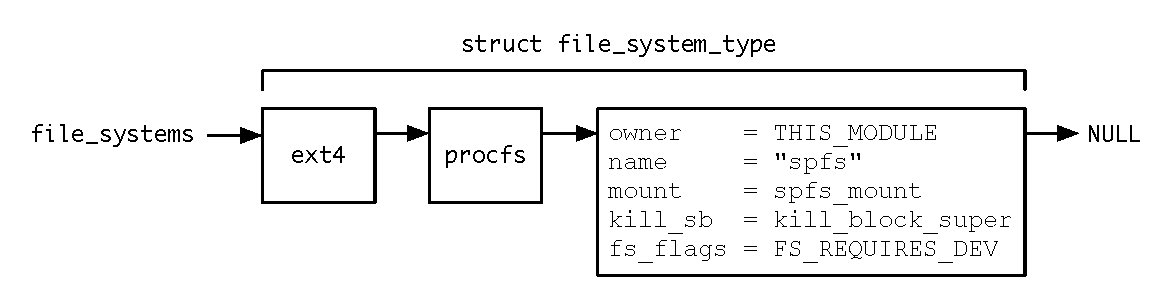
\includegraphics[scale=0.6]{figures/filesystems-available-expanded.pdf}
	\centering
	\caption{List of Available Filesystems}
	\label{fig:filesystems-available-expanded}
\end{figure}

\noindent
The main arguments of the \cf{struct file\_system\_type} are:

\begin{itemize}
	\item \cf{name} -- the name of the filesystem. When you run "\cf{mount -t spfs}", the kernel will
		compare "\cf{spfs}" against the \cf{name} field of each structure until a match is found or it 
		determines that this filesystem type does not exist or its corresponding modules has not
		been loaded.
	\item \cf{mount} -- the filesystem function which will be called during mount processing.
	\item \cf{kill\_sb} -- called when a filesystem is being unmounted.
\end{itemize}

\noindent
The filesystem \cf{kill\_sb()} function performs cleanup operations (freeing structures etc) and then invokes one of the following functions: \textbf{XXX---that's what the kernel doc says but some filesystems set kill\_sb to one of these functions. SPFS uses the first}

\begin{itemize}
	\item \cf{kill\_block\_super()} -- which unmounts a file system on a block device
	\item \cf{kill\_anon\_super()} -- which unmounts a virtual file system (information is generated when requested)
	\item \cf{kill\_litter\_super()} -- which unmounts a file system that is not on a physical device (the information 
			is kept in memory)
\end{itemize}

\noindent
You can run "\cf{cat /proc/filesystems}" to view the list of available filesystems. This will display all filesystems that are attached to \cf{file\_systems} as shown in figure \ref{fig:filesystems-available-expanded}. 

%--------------------------------------------------------------------------------------------------------------------------------------------------------

\subsection{The \cf{superblock} and \cf{mount} Structures}\label{superblock}

Once a filesystem is mounted, there is a \cf{super\_block} structure allocated for each mounted filesystem. The \cf{super\_blocks} variable points to a linked list of all mounted filesystems.

\begin{table}[h]
\begin{tabular}{ll}
\parbox[l]{0.6in}{
\includegraphics[scale=0.8]{figures/src-xref.pdf}} & \parbox[l]{4in}{\small{\cf{fs/superblocks.c} contains the \cf{super\_blocks} global variable which references all mounted filesystems. It also has routines for mounting and unmounting filesystems. The \cf{super\_block} structure can be found in \cf{include/linux/fs.h}}}
\end{tabular}
\end{table}

\noindent
There are a lot of fields in the \cf{super\_blocks}. A few are shown in figure \ref{fig:mount-structs} and described below:

\begin{figure}
	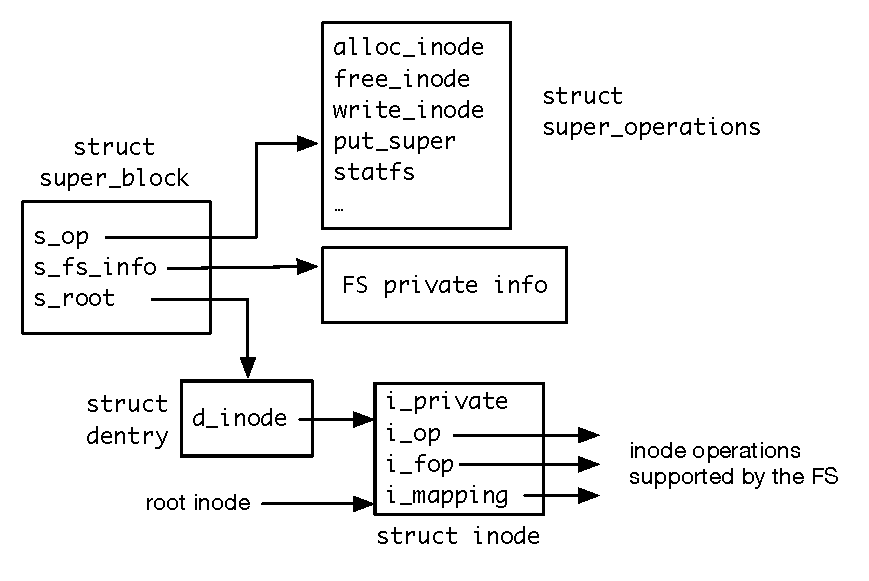
\includegraphics[scale=0.6]{figures/mount-structs.pdf}
	\centering
	\caption{Structures Representing Mounted Filesystems}
	\label{fig:mount-structs}
\end{figure}

\begin{itemize}
	\item \cf{s\_root} -- references the root dentry for this filesystem from which we can get to the root inode.
	\item \cf{s\_op} -- a set of filesystem-specific operations can can be invoked. Examples include
		inode operations such as allocation, writing (to disk) and freeing, writing the superblock to disk
		and reading per-filesystem stats (think \cf{df(1)}).
	\item \cf{s\_fs\_info} -- each filesystem will have information about this particular mount that it wishes to
		keep in-core. When a filesystem is mounted, the underlying filesystem can allocate such a structure
		and attach it to \cf{s\_fs\_info}.
	\item \cf{s\_dev} -- the device on which the filesystem resides. This will be accessed to read/write data
		through the buffer cache {\bfseries XXX etc - or is it s\_bdev???}.
\end{itemize}

\noindent
There are also several lists associated with each mount such as the list of dentries and several inode lists. {\bfseries XXX---expand etc}

\textbf{XXX---need to cover struct mount - see lx-mounts. also connection with vfsmount structure. not sure what the hell this is.}

\begin{lstlisting}
struct mount {
    struct hlist_node mnt_hash;
    struct mount *mnt_parent;
    struct dentry *mnt_mountpoint;
    struct vfsmount mnt;
\end{lstlisting}

\noindent
\textbf{Something about "mount"}

\begin{table}[h]
\begin{tabular}{ll}
\parbox[l]{0.6in}{
\includegraphics[scale=0.8]{figures/src-xref.pdf}} & \parbox[l]{4in}{\small{The \cf{mount} structure is defined in \cf{fs/mount.h} which differs from the \cf{mount.h} found in \cf{include/linux}.}}
\end{tabular}
\end{table}

%--------------------------------------------------------------------------------------------------------------------------------------------------------------

\subsection{The \cf{vfsmount} Structure}\label{kstruct-vfsmount}

XXX - need to add this too.

%-------------------------------------------------------------------------------------------------------------------------------------------------------------

\subsection{KGDB --- Analyzing the List of Mounted Filesystems}

This example shows how to view the list of mounted filesystems from within \cf{gdb}.

\begin{table}[h]
\begin{tabular}{ll}
\parbox[l]{0.6in}{
\includegraphics[scale=0.8]{figures/src-xref.pdf}} & \parbox[l]{4in}{\small{\cf{fs/proc\_namespace.c} contains code for the proc filesystem that deals with displaying mounted filesystems. The comment at the top of the file says \textit{but has rather close relationships with fs/namespace.c, thus here instead of fs/proc}}}
\end{tabular}
\end{table}

\noindent
The list of mounted filesystems is accessed through the \cf{super\_blocks} global variable (\cf{fs/super.c}) which is declared as follows: \textbf{XXX---the following link looks out of place}


\begin{lstlisting}
static LIST_HEAD(super_blocks);
\end{lstlisting}

\noindent
Locating this variable in \cf{gdb} gives us:

\begin{lstlisting}
(gdb) [*\bfseries p super\_blocks*]
$56 = {
  next = 0xffff0000c0022800,
  prev = 0xffff0000e4455000
}
\end{lstlisting}

\noindent
A simple way to view all of the mounted filesystems is to use the Linux helper function \cf{lx\_mounts} which displays information for all mounted filesystems. You can then display more information about each mounted filesystem given the addresses of the \cf{mount} and \cf{super\_block} structure addresses displayed.

\begin{lstlisting}
(gdb) [*\bfseries  lx-mounts*]
      mount          super_block      devname pathname fstype
[*\bfseries 0xffff0000c0285540 0xffff0000c0025000*] rootfs  /        rootfs 
0xffff0000c0835900 0xffff0000c08a5000 sysfs   /sys     sysfs
0xffff0000c0834780 0xffff0000c08a7800 proc    /proc    proc
...
\end{lstlisting}

\noindent
For the first row (highlighted), let's see how these structures are connected. First we show the link from the \cf{mount} structure to the \cf{super\_block} structure:

\begin{lstlisting}
(gdb)  [*\bfseries set \$mount = (struct mount *)0xffff0000c0285540*]
(gdb)  [*\bfseries p \$mount->mnt.mnt\_sb*]
$5946 = (struct super_block *) 0xffff0000c0025000
\end{lstlisting}

\noindent
The mount point can also be displayed:

\begin{lstlisting}
(gdb)  [*\bfseries p \$mount->mnt\_mountpoint->d\_name.name*]
$5948 = (const unsigned char *) 0xffff0000c0404f38 "/"
\end{lstlisting}

\noindent
For another filesystem:

\begin{lstlisting}
$ [*\bfseries mount | grep spfs*]
/dev/sda on /mnt type spfs (rw,relatime)
\end{lstlisting}

\noindent
we display the mount point and the name of the device:

\begin{lstlisting}
(gdb) [*\bfseries pipe lx-mounts | grep spfs*]
0xffff0000d9e5da40 0xffff0000e4455000 /dev/sda /mnt spfs ...
(gdb) [*\bfseries set \$mount = (struct mount *)0xffff0000d9e5da40*]
(gdb) [*\bfseries p \$mount->mnt\_mountpoint->d\_name.name*]
$5955 = (const unsigned char *) 0xffff0000f3fbaf38 "mnt"
(gdb) [*\bfseries p \$mount->mnt\_devname*]
$5956 = 0xffff0000e622e200 "/dev/sda"
\end{lstlisting}

\noindent
\textbf{Need to bring in vfsmount and perhaps show a figure or add a figure earlier. Seems like a bug dump}

%%%%%%%%%%%%%%%%%%%%%%%%%%%%%%%%%%%%%%%%%%%%%%%%%%%%%%%%%%%%%%%%

\section{Namespace Structures}

% https://blog.quarkslab.com/digging-into-linux-namespaces-part-2.html - good example to get started

The \cf{mount\_namespaces(7)} manpage gives a good introduction to mount namespaces. 

The \cf{unshare(1)} command runs a program in a new namespace. 

The \cf{user\_namespace} structure needs some explaining. Here is a subset of the structure:

\begin{lstlisting}
struct user_namespace {
    struct uid_gid_map   uid_map;
    struct uid_gid_map   gid_map;
    struct uid_gid_map   projid_map;
    struct user_namespace  *parent;
    int                     level;
    kuid_t                  owner;
    kgid_t                  group;
    struct ns_common        ns;
    unsigned long           flags;
    bool                    parent_could_setfcap;
    struct work_struct      work;
    struct ucounts         *ucounts;
    long                    ucount_max[UCOUNT_COUNTS];
    long                    rlimit_max[UCOUNT_RLIMIT_COUNTS];
}
\end{lstlisting}

\noindent
Inside the \cf{super\_block} structure there is a field that references namespaces:

\begin{lstlisting}
struct user_namespace *s_user_ns;
\end{lstlisting}

\noindent
There are 60 references to this all over the place!!!

%%%%%%%%%%%%%%%%%%%%%%%%%%%%%%%%%%%%%%%%%%%%%%%%%%%%%%%%%%%%%%%

\section{Conclusion}

This chapter provided a lot of information starting with tools to help you explore the Linux kernel which is now over 26 million lines of code so somewhat daunting especially if you haven't looked at the kernel before or looked at much earlier versions.

This chapter started to dig into the Linux kernel. The first step is to get familiar with navigating around the kernel source so tools were presented to show how to navigate around the source code in addition to inline cross reference tools. Although there are over 26 million LOC in the kernel, the filesystem components are only found in a small number of places so browsing becomes a little easier.

The book has been following a path from user libraries through the system call handling and into the individual filesystems. The system call layer was explained and showed how to find system call handler for its respective system call functions that applications invoke. From there it's possible to navigate through the file handling kernel code.

There are several subsystems that comprise filesystem access including the directory cache, buffer cache, page cache and inode caches. Each of these subsystems were described showing how they are all interconnected. Before digging into the filesystem kernel paths in the next chapter, it's imperative to have an understanding of what these components deliver.

The main structures used for file and filesystem access were described showing how they link together. To help reinforce the material, kernel debugging using \cf{gdb} was introduced and several examples were shown to highlight how the structures are linked together. Other examples made us of the \cf{crash(1)} utility. This should provide you with enough information to be able to explore how the kernel structures are linked together. It's recommended to try the examples shown here, look at the other fields of the structures displayed and try different examples.


